\chapter{Results}\label{ch:results}
Presented here are a number of test cases which access the accuracy of the matrix exponential solvers in libowski. The majority of analysis thus far is done on what is known as Problem 1. Two major properties which influence the accuracy of each method are exploited, matrix norm and eigenvalues with both time stepping methods. There are also verification problems for diffusion and convection problems to test the spatial and temporal accuracy. Finally there is a neutron precursor problem showing the application in a nuclear reactor type test problem. 

\section{Problem 1}
This test contains two variations of the same three isotope decay problem shown in Equation \ref{eq:problem1}. In each problem, the decay constants are changed to induce different eigenvalues.

\begin{equation}
\begin{split}
    \frac{dN_{1}}{dt} &= \lambda_{3}N_{3} - \lambda_{1}N_{1}, \quad N_{1}(0) = 10000\\
    \frac{dN_{2}}{dt} &= \lambda_{1}N_{1} - \lambda_{2}N_{2}, \quad N_{2}(0) = 0\\
    \frac{dN_{3}}{dt} &= \lambda_{2}N_{2} - \lambda_{3}N_{3}, \quad N_{3}(0) = 0
\end{split}
    \label{eq:problem1}
\end{equation}

Problem 1a induces only real eigenvalues $[0, -0.02, -0.025]$ and $||A||_{l_{1}} =0.06$ when $t=1$ and linearly increases to $36$ when $t_{end}=600$. The corresponding decay constants are $[\lambda_{1}, \lambda_{2}, \lambda_{3}] = [0.1, 0.005, 0.03]$. Both time marching methods are tested against an analytical solution which was generated in Matlab. 

\begin{table}[b]
    \caption{\label{tab:results1a} Problem 1a $l_{\infty}$ Error for Time Marching Scheme 1}
    \centering
    %\begin{tabular}{c|p{1.5cm}|p{1.5cm}|p{1.5cm}|p{1.5cm}|p{1.5cm}|p{1.5cm}}
    \begin{tabular}{c|c|c|c}
    \hline
     & $N_{1}$ & $N_{2}$ & $N_{3}$ \\
    \hline
    \hline
    CRAM & 7.28E-12 & 5.46E-12 & 2.39E-12 \\
    \hline
    Parabolic & 6.37E-11 & 6.46E-11 & 2.40E-11 \\
    \hline
    Hyperbolic & 7.28E-12 & 4.09E-12 & 1.40E-12 \\
    \hline
    Pad\'e Method 1 & 7.73E-12 & 1.27E-11 & 2.16E-12 \\
    \hline
    Pad\'e Method 2 & 7.73E-12 & 1.27E-11 & 2.16E-12 \\
    \hline
    \end{tabular}
\end{table}

Results for time marching scheme 1 were generated by taking one time step to $t_{end} = 600$. Table \ref{tab:results1a} shows that the Hyperbolic solver outperforms all other solvers for isotopes 2 and 3 while performs as well as the CRAM solver for isotope 1. Both Pad\'e methods gives the same $l_{\infty}$ error for each isotope and is only slightly larger than the minimum error for isotope 1. The Parabolic solver has the worst error for all isotopes. 

Test are conducted with time marching scheme 2 at various time steps for each solver. The $l_{\infty}$ error for each isotope are is shown in Figure \ref{fig:errorProblem1aTimeMarchingScheme2}. Error for each of the Cauchy solvers exponentially decays as you decrease the number of substeps (increase the time step size) you take as your march to $t_{end}=600$. Because the isotope concentrations do not sharply decrease as steady state is reached, substeping a Cauchy solver will not increase the accuracy. The reason the accuracy decreases was described in Section \ref{sec:timeMarchingSchemes}. In general, the Pad\'e solvers also follows this trend although it is not as sharp as the Cauchy solvers. Pad\'e-Method 1 shows a sharp increase in error after the first time step size then tends to decrease with few small increases in error between a number of time steps. These small increases might be cause by the matrix norm increases but not enough to jump to a higher order Pad\'e function. When the norm increases over that Pad\'e orders threshold, the error sharply jumps down because a higher order Pad\'e method is used to approximation the matrix exponential. After a point the matrix norm becomes too large, and squaring a scaling takes place. 


\begin{figure}[t]
  \centering
  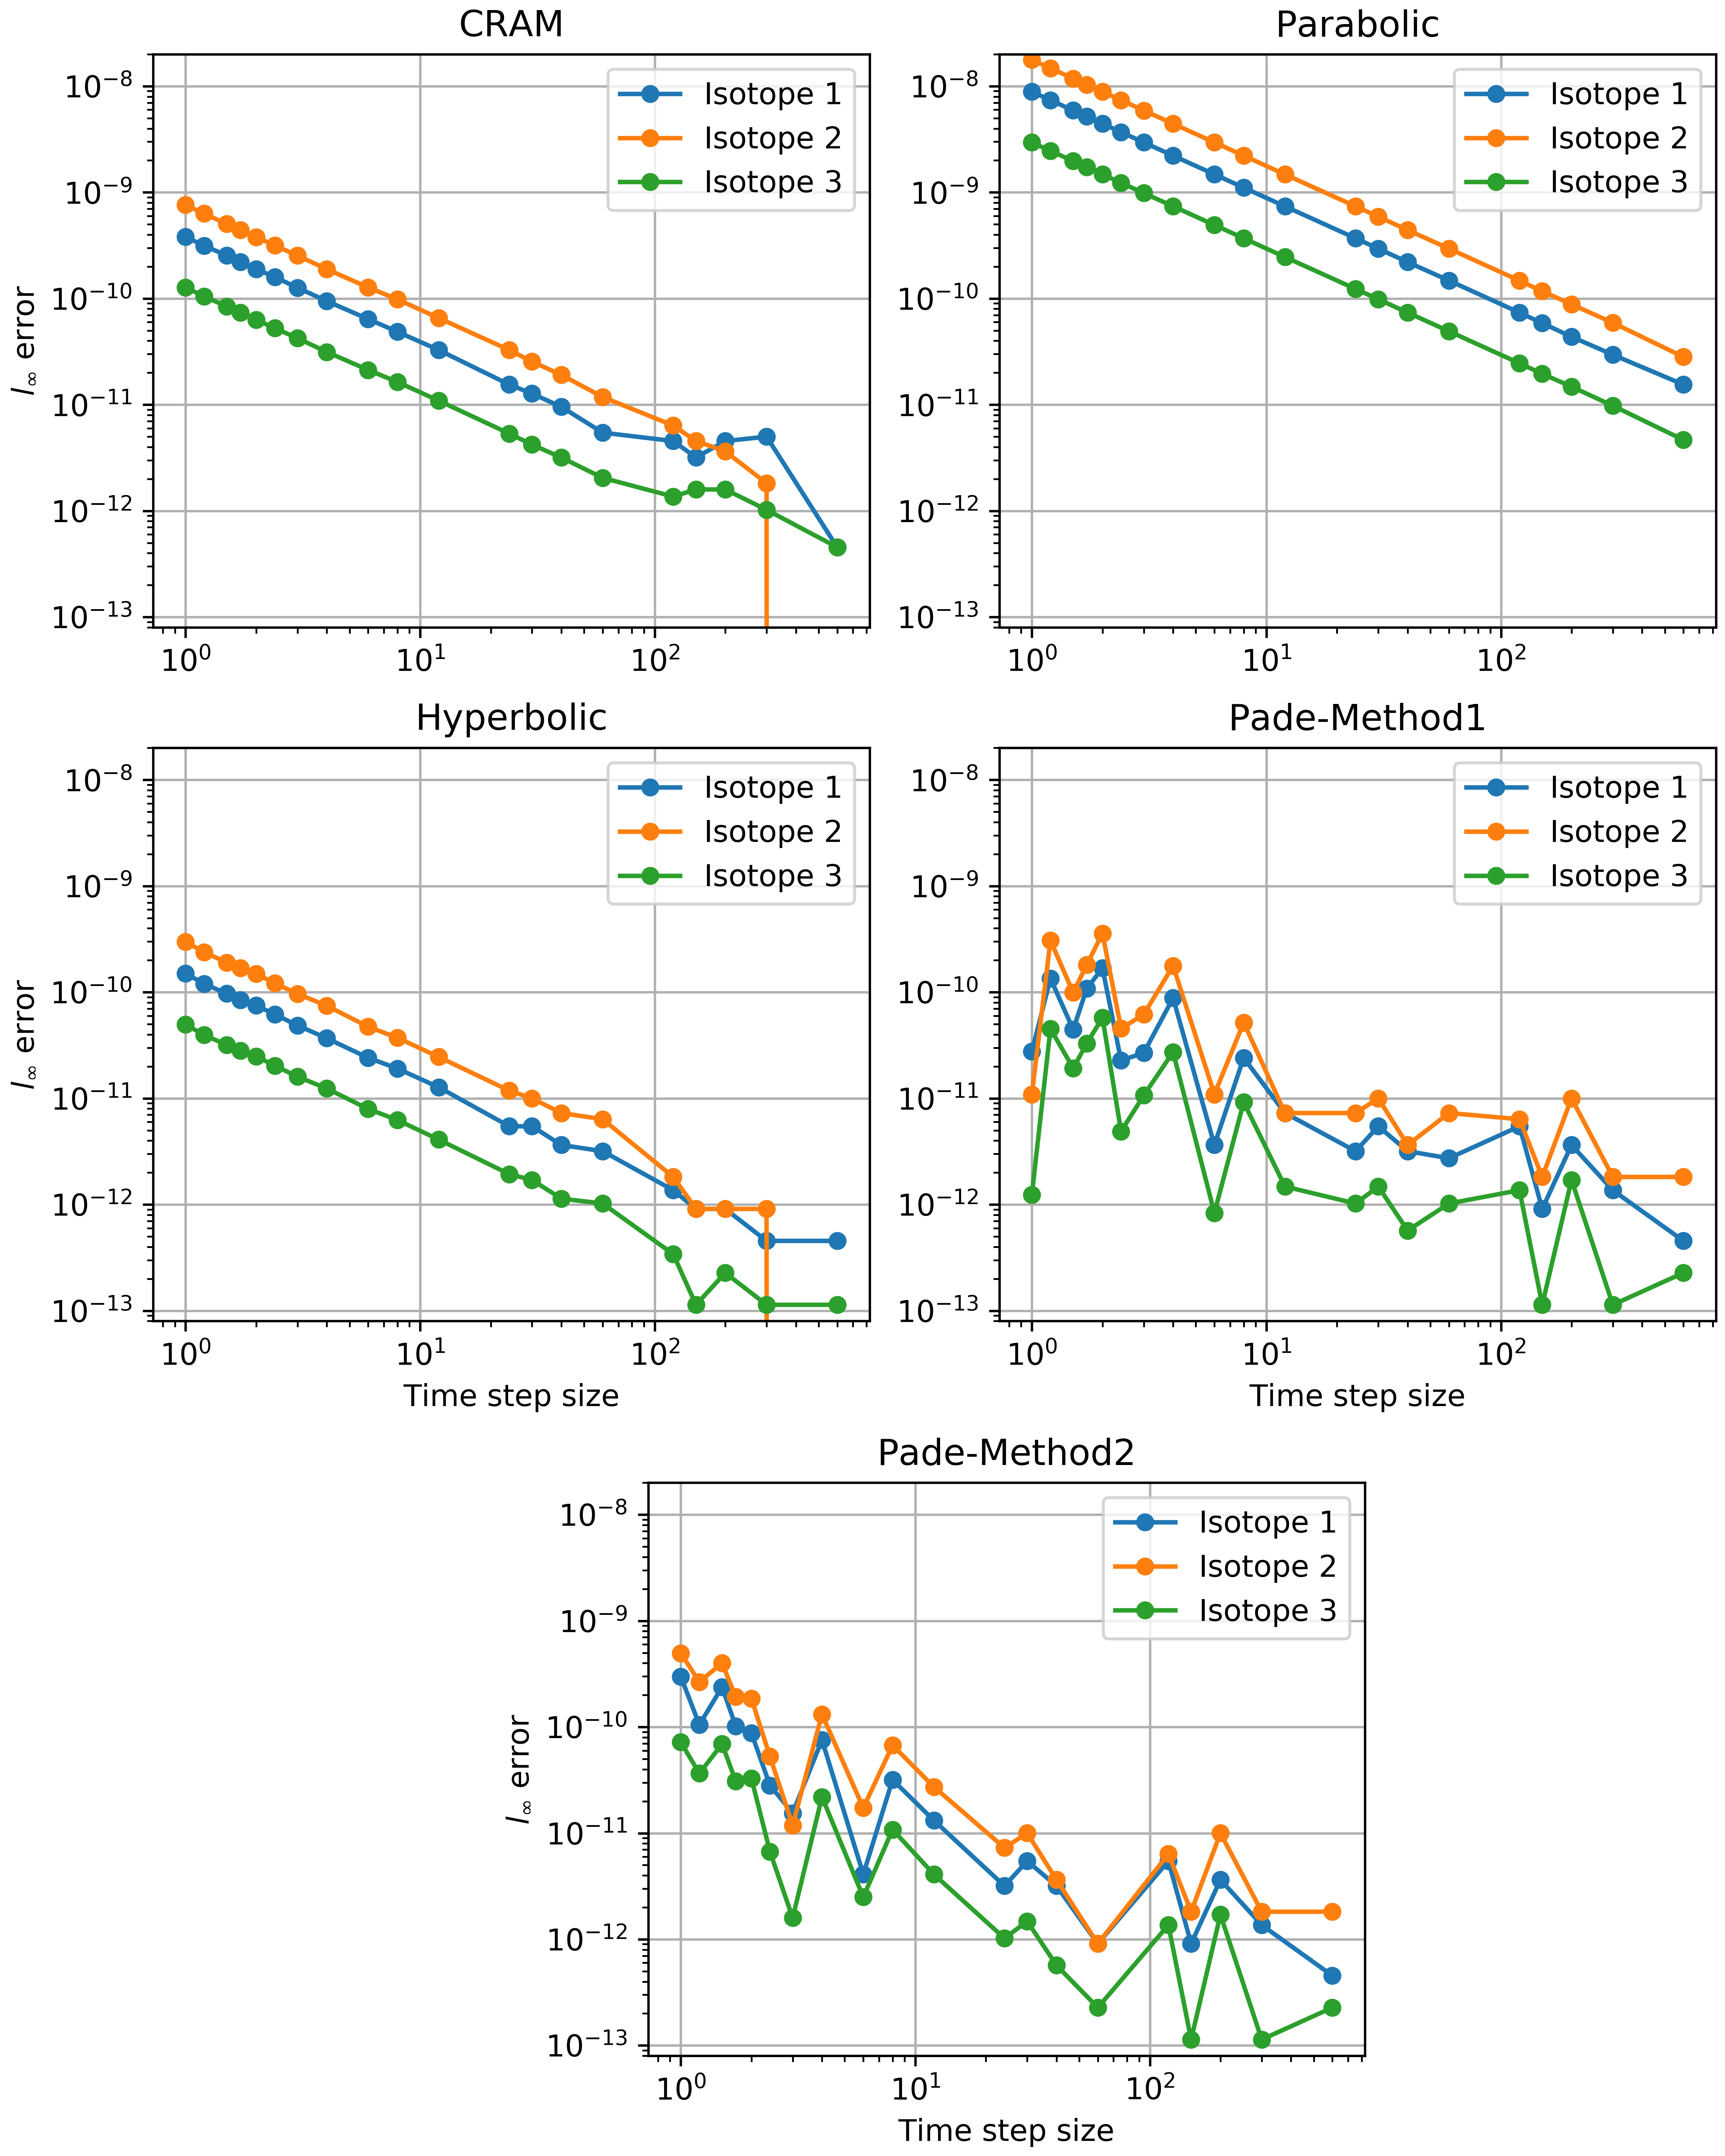
\includegraphics[width=6.5in]{images/problem1aMethod2.png}\\
  \caption{Error for Problem 1a Using Time Marching Scheme 2}
  \label{fig:errorProblem1aTimeMarchingScheme2}
\end{figure} 

\FloatBarrier



Problem 1b modifies the decay constants to produce eigenvalues with imaginary parts [2.05e-19, -1.5e-02+0.00707107i, -1.5e-02-0.00707107i] with $||A||_{l_{1}} = 0.03$ when $t=1$ and linearly increases to 18 when $t_{end} = 600.$ The corresponding decay constants are $[\lambda_{1}, \lambda_{2}, \lambda_{3}] = [0.1, 0.005, 0.105]$. Again, the solution was generated in Matlab. 

Results for time marching scheme 1 were generated by taking one time step to $t_{end} = 600$. Table \ref{tab:results1b} shows that CRAM was the worst preforming solver. This is not surprising considering the magnitude of the imaginary parts of the eigenvalues, CRAM is most accurate around the negative real axis. Both Parabolic and Hyperbolic solvers cover a wider range on the imaginary axis, which shows in the results. Each of these solvers are many orders of magnitude more accurate than CRAM. The Pad\'e solvers both give the same solution, this is not surprising because there are situations in Pad\'e Method 2 which will run as Method 1. Again the Hyperbolic solver is the most accurate.

Results for time marching scheme 2 are shown in Figure \ref{fig:errorProblem1aTimeMarchingScheme2} and shows one of the advantages of substepping. As the time step length increases, so do the placement of the eigenvalues on the complex plane. If the time step is too large, the eigenvalues can shift into a region which decreases the accuracy of Cauchy methods; this behavior is most prevalent in CRAM. Both the Parabolic and Hyperbolic solvers also show a slight bump in error after time steps on the order of 100, after the error starts to decline again and bottoms out at the last point. The last point corresponds to taking a single time step. Both of the Pad\'e solvers show the same general trend as with problem 1a. The matrix norm for this problem is slightly lower than with problem 1a, leading to lower error. 

\begin{table}[b]
    \caption{\label{tab:results1b} Problem 1b $l_{\infty}$ Error for Time Marching Scheme 1}
    \centering
    %\begin{tabular}{c|p{1.5cm}|p{1.5cm}|p{1.5cm}|p{1.5cm}|p{1.5cm}|p{1.5cm}}
    \begin{tabular}{c|c|c|c}
    \hline
     & $N_{1}$ & $N_{2}$ & $N_{3}$ \\
    \hline
    \hline
    CRAM & 5.73E-9 & 4.37E-9 & 1.36E-9 \\
    \hline
    Parabolic & 8.64E-11 & 9.09E-12 & 1.26E-10 \\
    \hline
    Hyperbolic & 9.09E-13 & 9.09E-13 & 6.82E-13 \\
    \hline
    Pad\'e Method 1 & 1.36E-12 & 9.09E-13 & 2.27E-13 \\
    \hline
    Pad\'e Method 2 & 1.36E-12 & 9.09E-13 & 2.27E-13 \\
    \hline
    \end{tabular}
\end{table}

\begin{figure}[t]
  \centering
  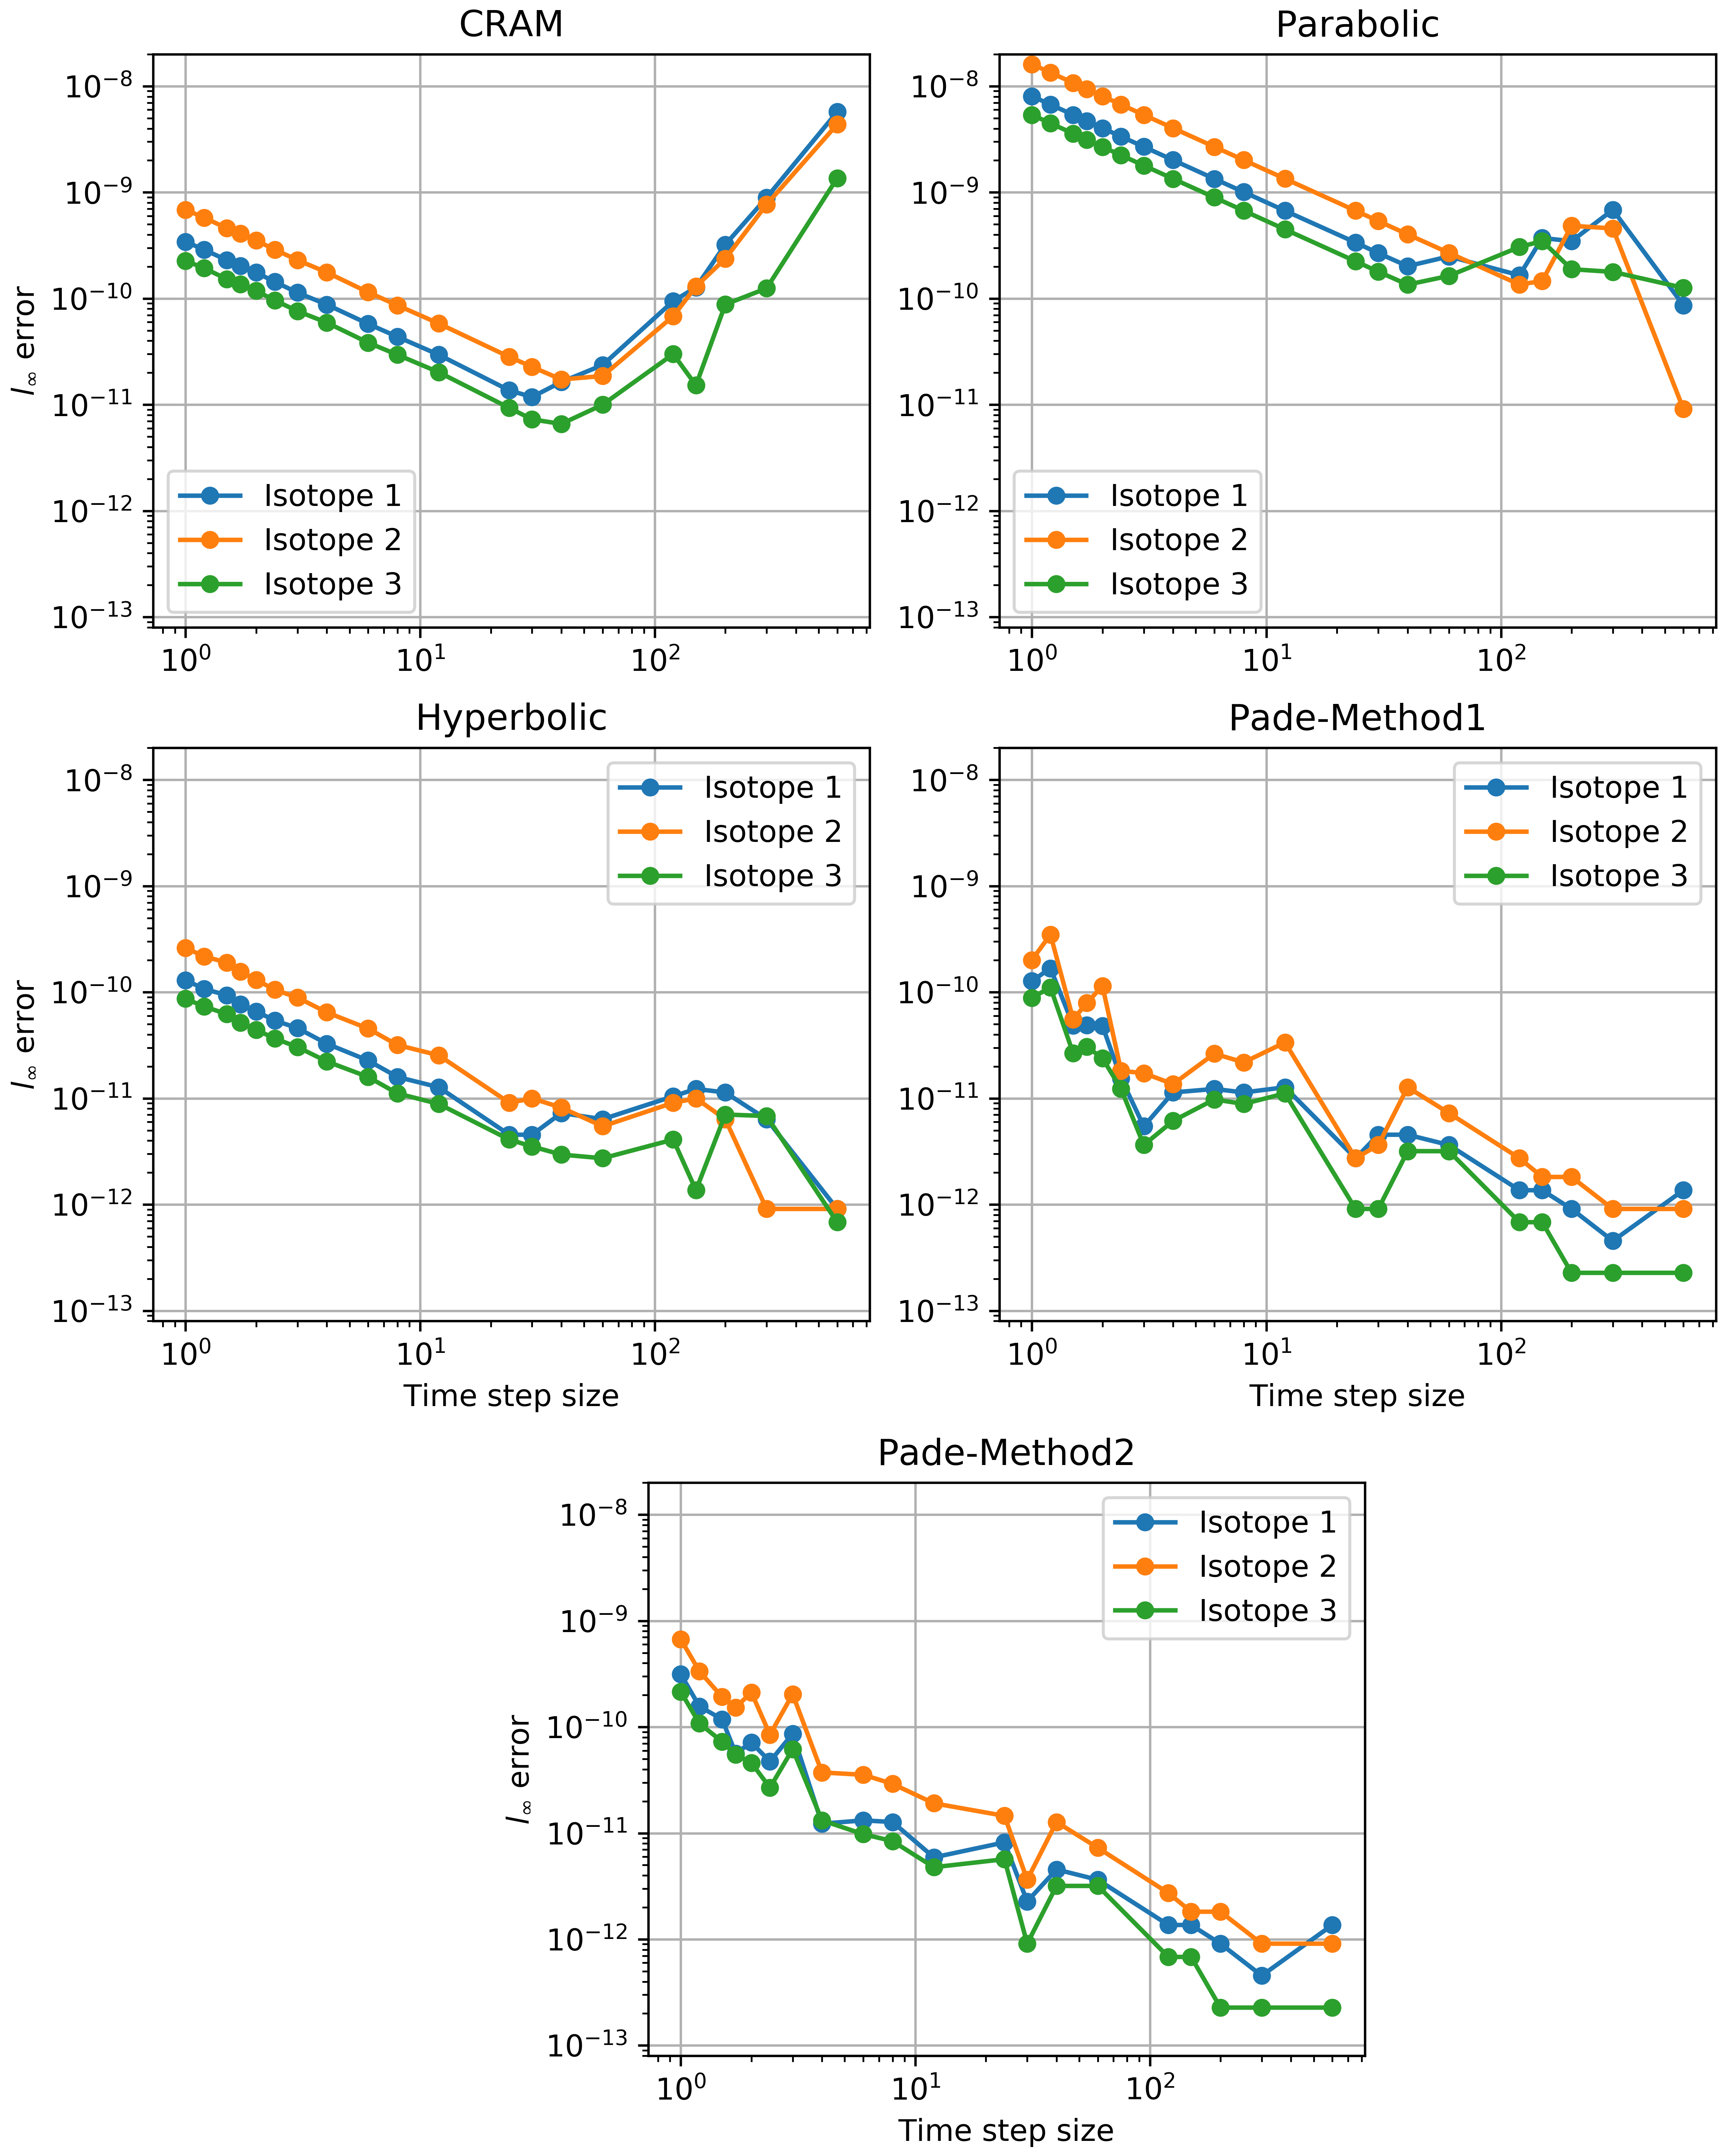
\includegraphics[width=6.5in]{images/problem1bMethod2.png}\\
  \caption{Error for Problem 1b Using Time Marching Scheme 2}
  \label{fig:errorProblem1aTimeMarchingScheme2}
\end{figure} 

\FloatBarrier

\section{Problem 2}
Problem 2 is a 1D, two species reaction-diffusion problem shown in Equation \ref{eq:problem2Eqs} \cite{ching2007},

\begin{equation}
\setlength{\jot}{15pt}
\begin{split}
    \frac{\partial U}{\partial t} &= d\frac{\partial^{2}U}{\partial x^{2}} - aU + V, \\
    \frac{\partial V}{\partial t} &=
    d\frac{\partial^{2}V}{\partial x^{2}} - bV,
\end{split}
    \label{eq:problem2Eqs}
\end{equation}

\noindent on the domain from $0$ to $\pi/2$. The system is subject to the following boundary conditions, 

\begin{equation}
    \frac{\partial U}{\partial x}(0,t) = 0, \quad \frac{\partial V}{\partial x}(0,t) = 0, \quad U(\frac{\pi}{2}, t) = 0, \quad V(\frac{\pi}{2}, t)= 0,
\end{equation}

\noindent with initial condition,

\begin{equation}
    U(x,0) = 2\cos(x), \quad V(x,0) = (a-b)\cos(x).
\end{equation}

\noindent The exact solution is given by,

\begin{equation}
    U(x,t) = \bigg( e^{-(a+d)t} + e^{-(b+d)t}\bigg)\cos(x), \quad V(x,t) = (a - b) e^{-(b+d)t}\cos(x).
\end{equation}

The same three test problems that were conducted in Reference \cite{ching2007} are also done in libowski. These test correspond to changes in coefficients $[a, b, d]$ which produce a diffusion dominated system, a reaction dominated system and a stiff reaction system. Each test case is run with one time step to $t = 1$, so $\Delta t = 1$. The number of cells in the x-direction is varied from 100 to 1000. In addition to the five matrix exponential solvers that are tested, the Krylov subspace approximation is applied to both of the Pad\'e solvers with the aim to reduce the solve time. 

Results for each of the five solvers are shown in Figures \ref{fig:errorProblem2CRAM} to \ref{fig:errorProblem2padeM2}. The errors for each of the test cases is almost the same for each of the solvers. What is most interesting is that the error for $U$ remains pretty constant for each test case however, the error for V drastically changes. Test case one is a diffusion dominating problem were $V$ is weakly dependent on $U$. The error in $V$ for this case is an order of magnitude lower than $U$. In test case two, the coupling between the two species is the came order of magnitude and is reflected in the error. In this case the problem is reaction dominated. The third test case is also reaction dominated but with stiff reaction rates. Species $U$ decays at a rate that is 2 orders of magnitude greater than in test case two. This is reflected not in the $U$ solution but in the $V$ solution which is about two orders of magnitude more error. 

The most notable difference between the solvers is their run time. Each of the Cauchy solvers have run times of less than $0.1$ seconds, even for the smallest dx, corresponding to a 2000 x 2000 matrix. Both the Parabolic and Hyperbolic solvers require twice as many linear solves as CRAM, resulting in about twice the run time. The run time for Cauchy class solvers also scales by about 2 orders of magnitude from the largest dx to the smallest dx. Both of the Pad\'e solvers have much larger differences in run time as dx scales down in size, corresponding to 5 about orders of magnitude in solve time. At the problems highest spatial resolution, Pad\'e solvers take about 100 seconds to solve vs 0.05 seconds for Caunchy solvers. 

The Krylov subspace method is applied to the Pad\'e solvers to reduce their computation time. Testing each case was accomplished by selecting a base discritization resulting from 800 cells in the x-direction. Next, Krylov subspaces of various dimensions are built from the original 1600 x 1600 matrix. Results for each of the Pad\'e solvers are shown in Figures \ref{fig:errorProblem2padeM1Krylov} and \ref{fig:errorProblem2padeM2Krylov}. In each test case, a Krylov dimension is reached where the original base error from the 1600 x 1600 matrix. In the diffusion dominated case this optimal Krylov dimension is 50, meaning that the original 1600 x 1600 problem can be reduced to a 50 x 50 matrix and solved with the same solution error. For case one, this reduces the computation time from $\sim35$ seconds to $\sim 10^{-2}$ seconds. The benefit from the Krylov subpsace method is even more prevalent in the reaction dominated cases. In both of these cases, a subpsace dimension of only 3 is required to reach the same base error for the 1600 x 1600 matrix. This reduces the computation time from $\sim 35$ seconds to $\sim 5\times 10^{-4}$ seconds. 

%Doing so allows for the comparison of libowski to the IF2 solver that was developed in Reference \cite{ching2007}. 

\FloatBarrier

\begin{figure}[t]
  \centering
  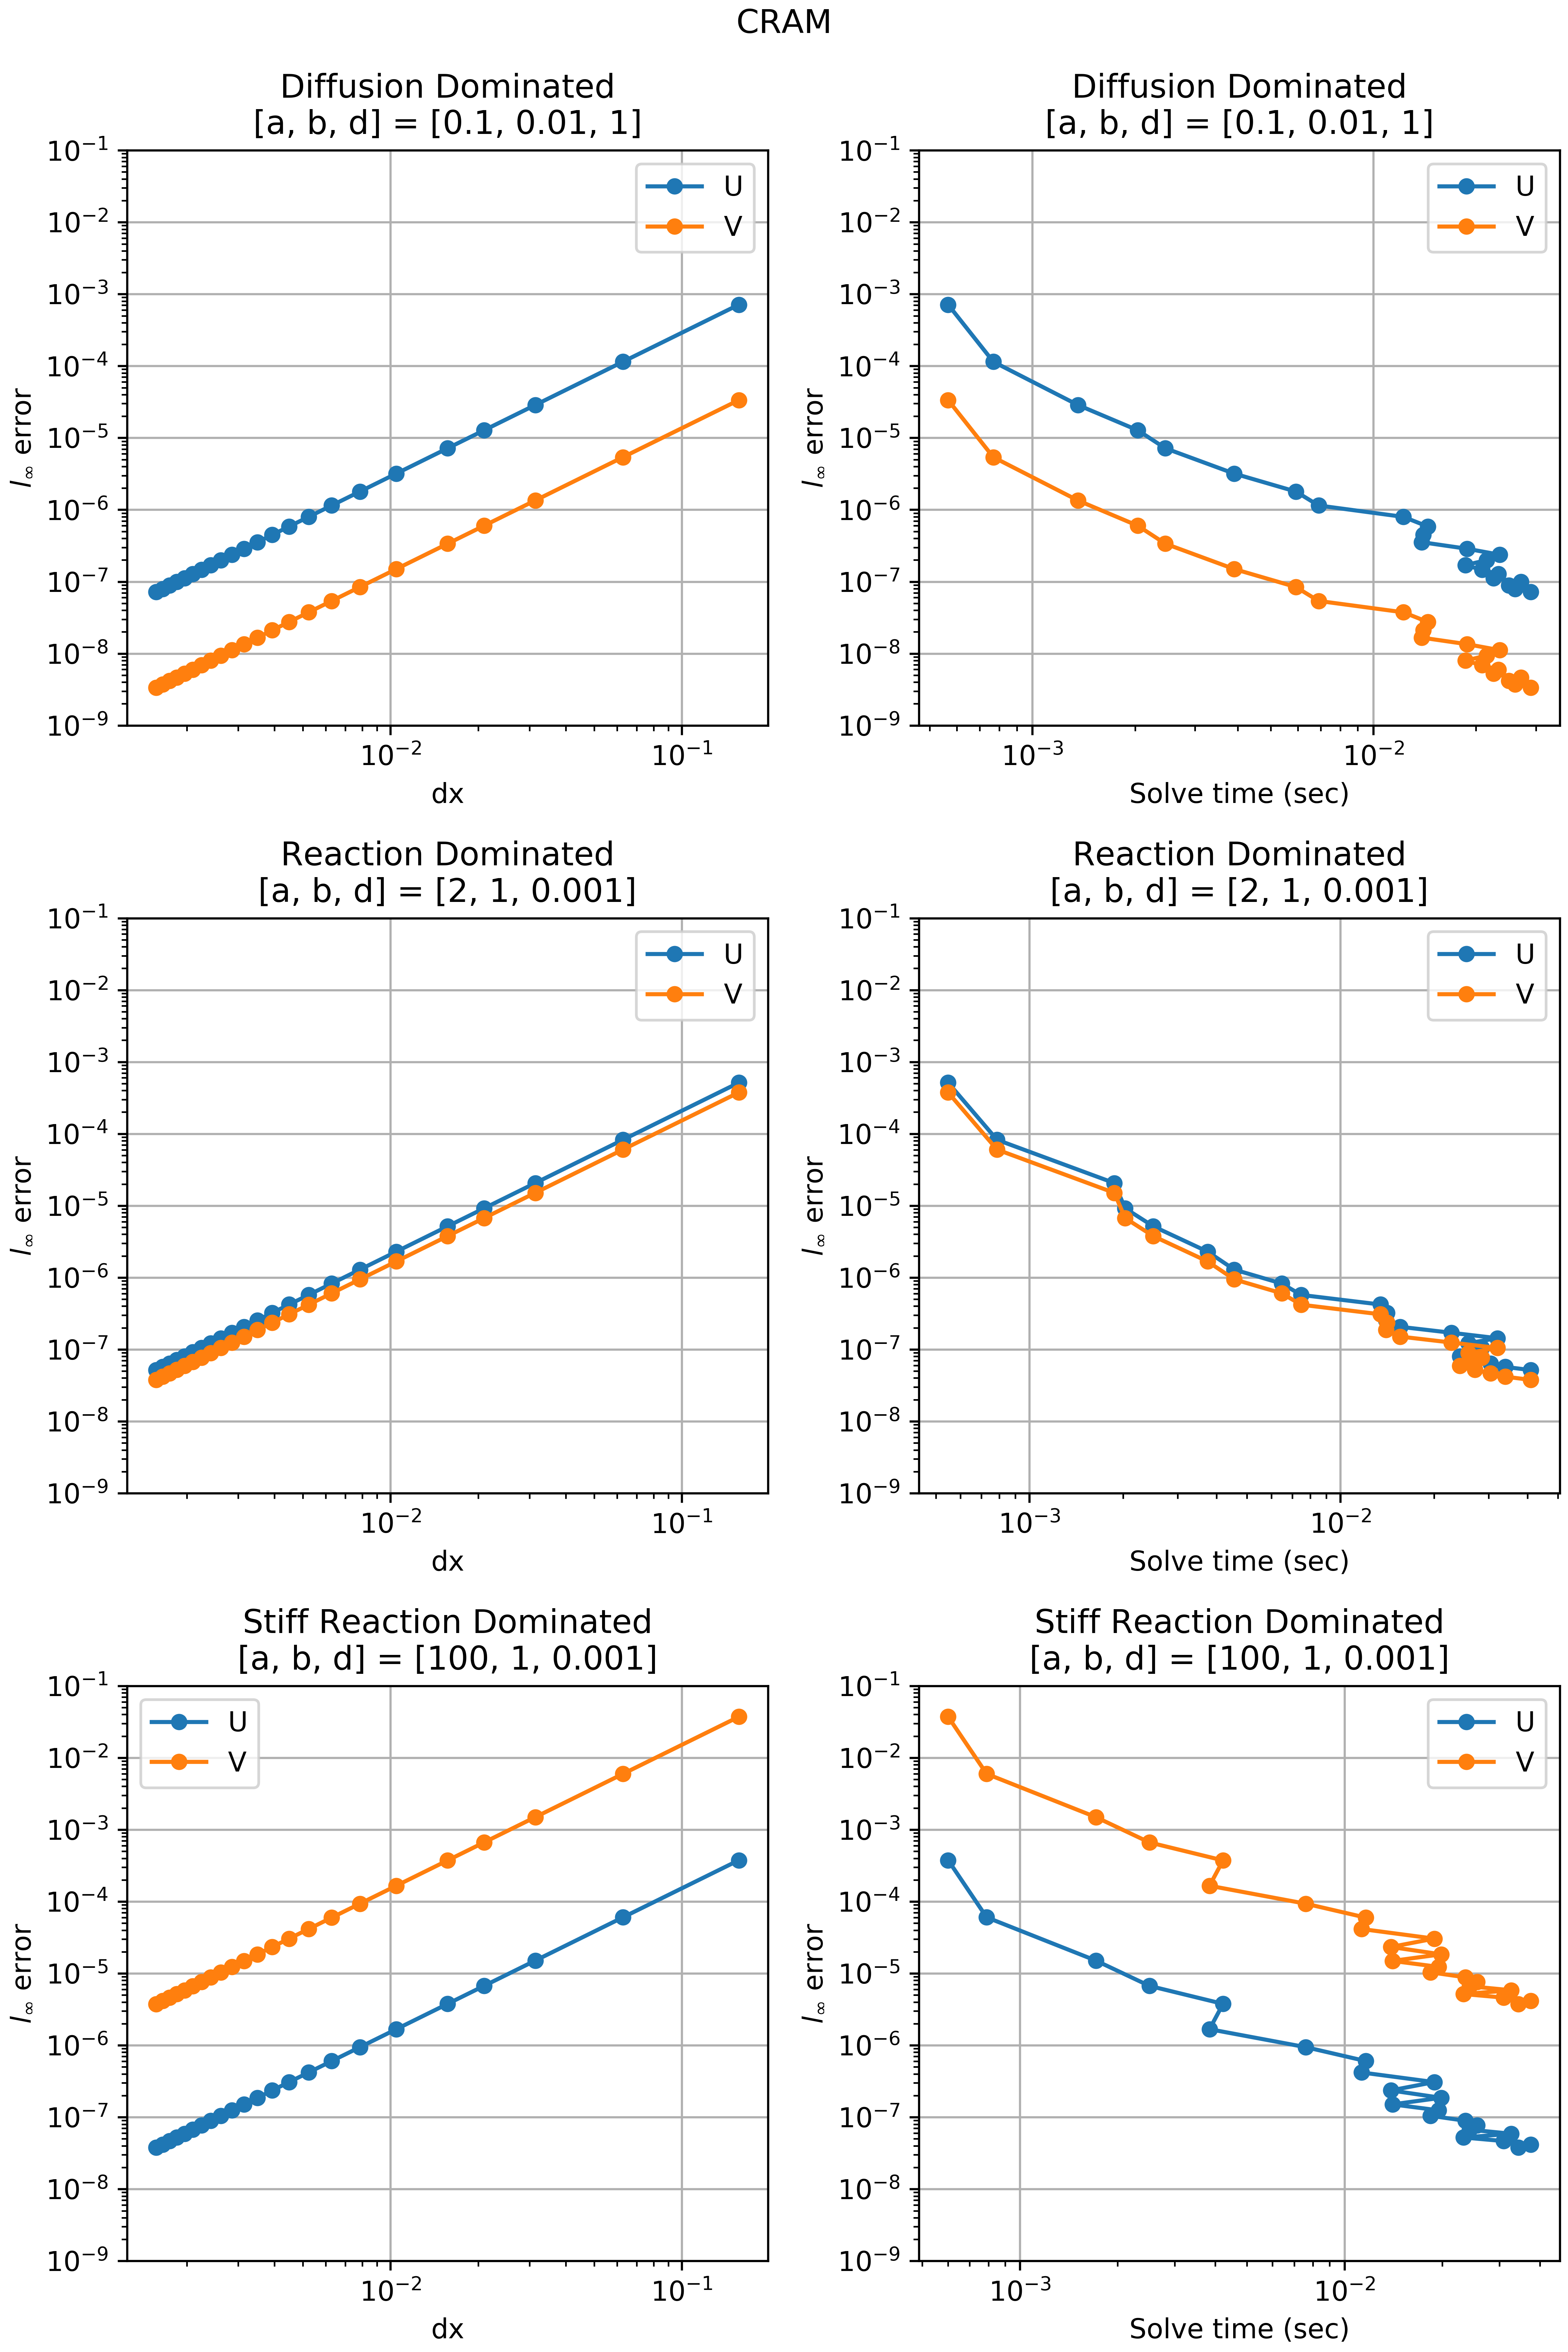
\includegraphics[width=5.75in]{images/CRAMproblem2.png}\\
  \caption{Error for Problem 2 Using CRAM}
  \label{fig:errorProblem2CRAM}
\end{figure} 


\begin{figure}[t]
  \centering
  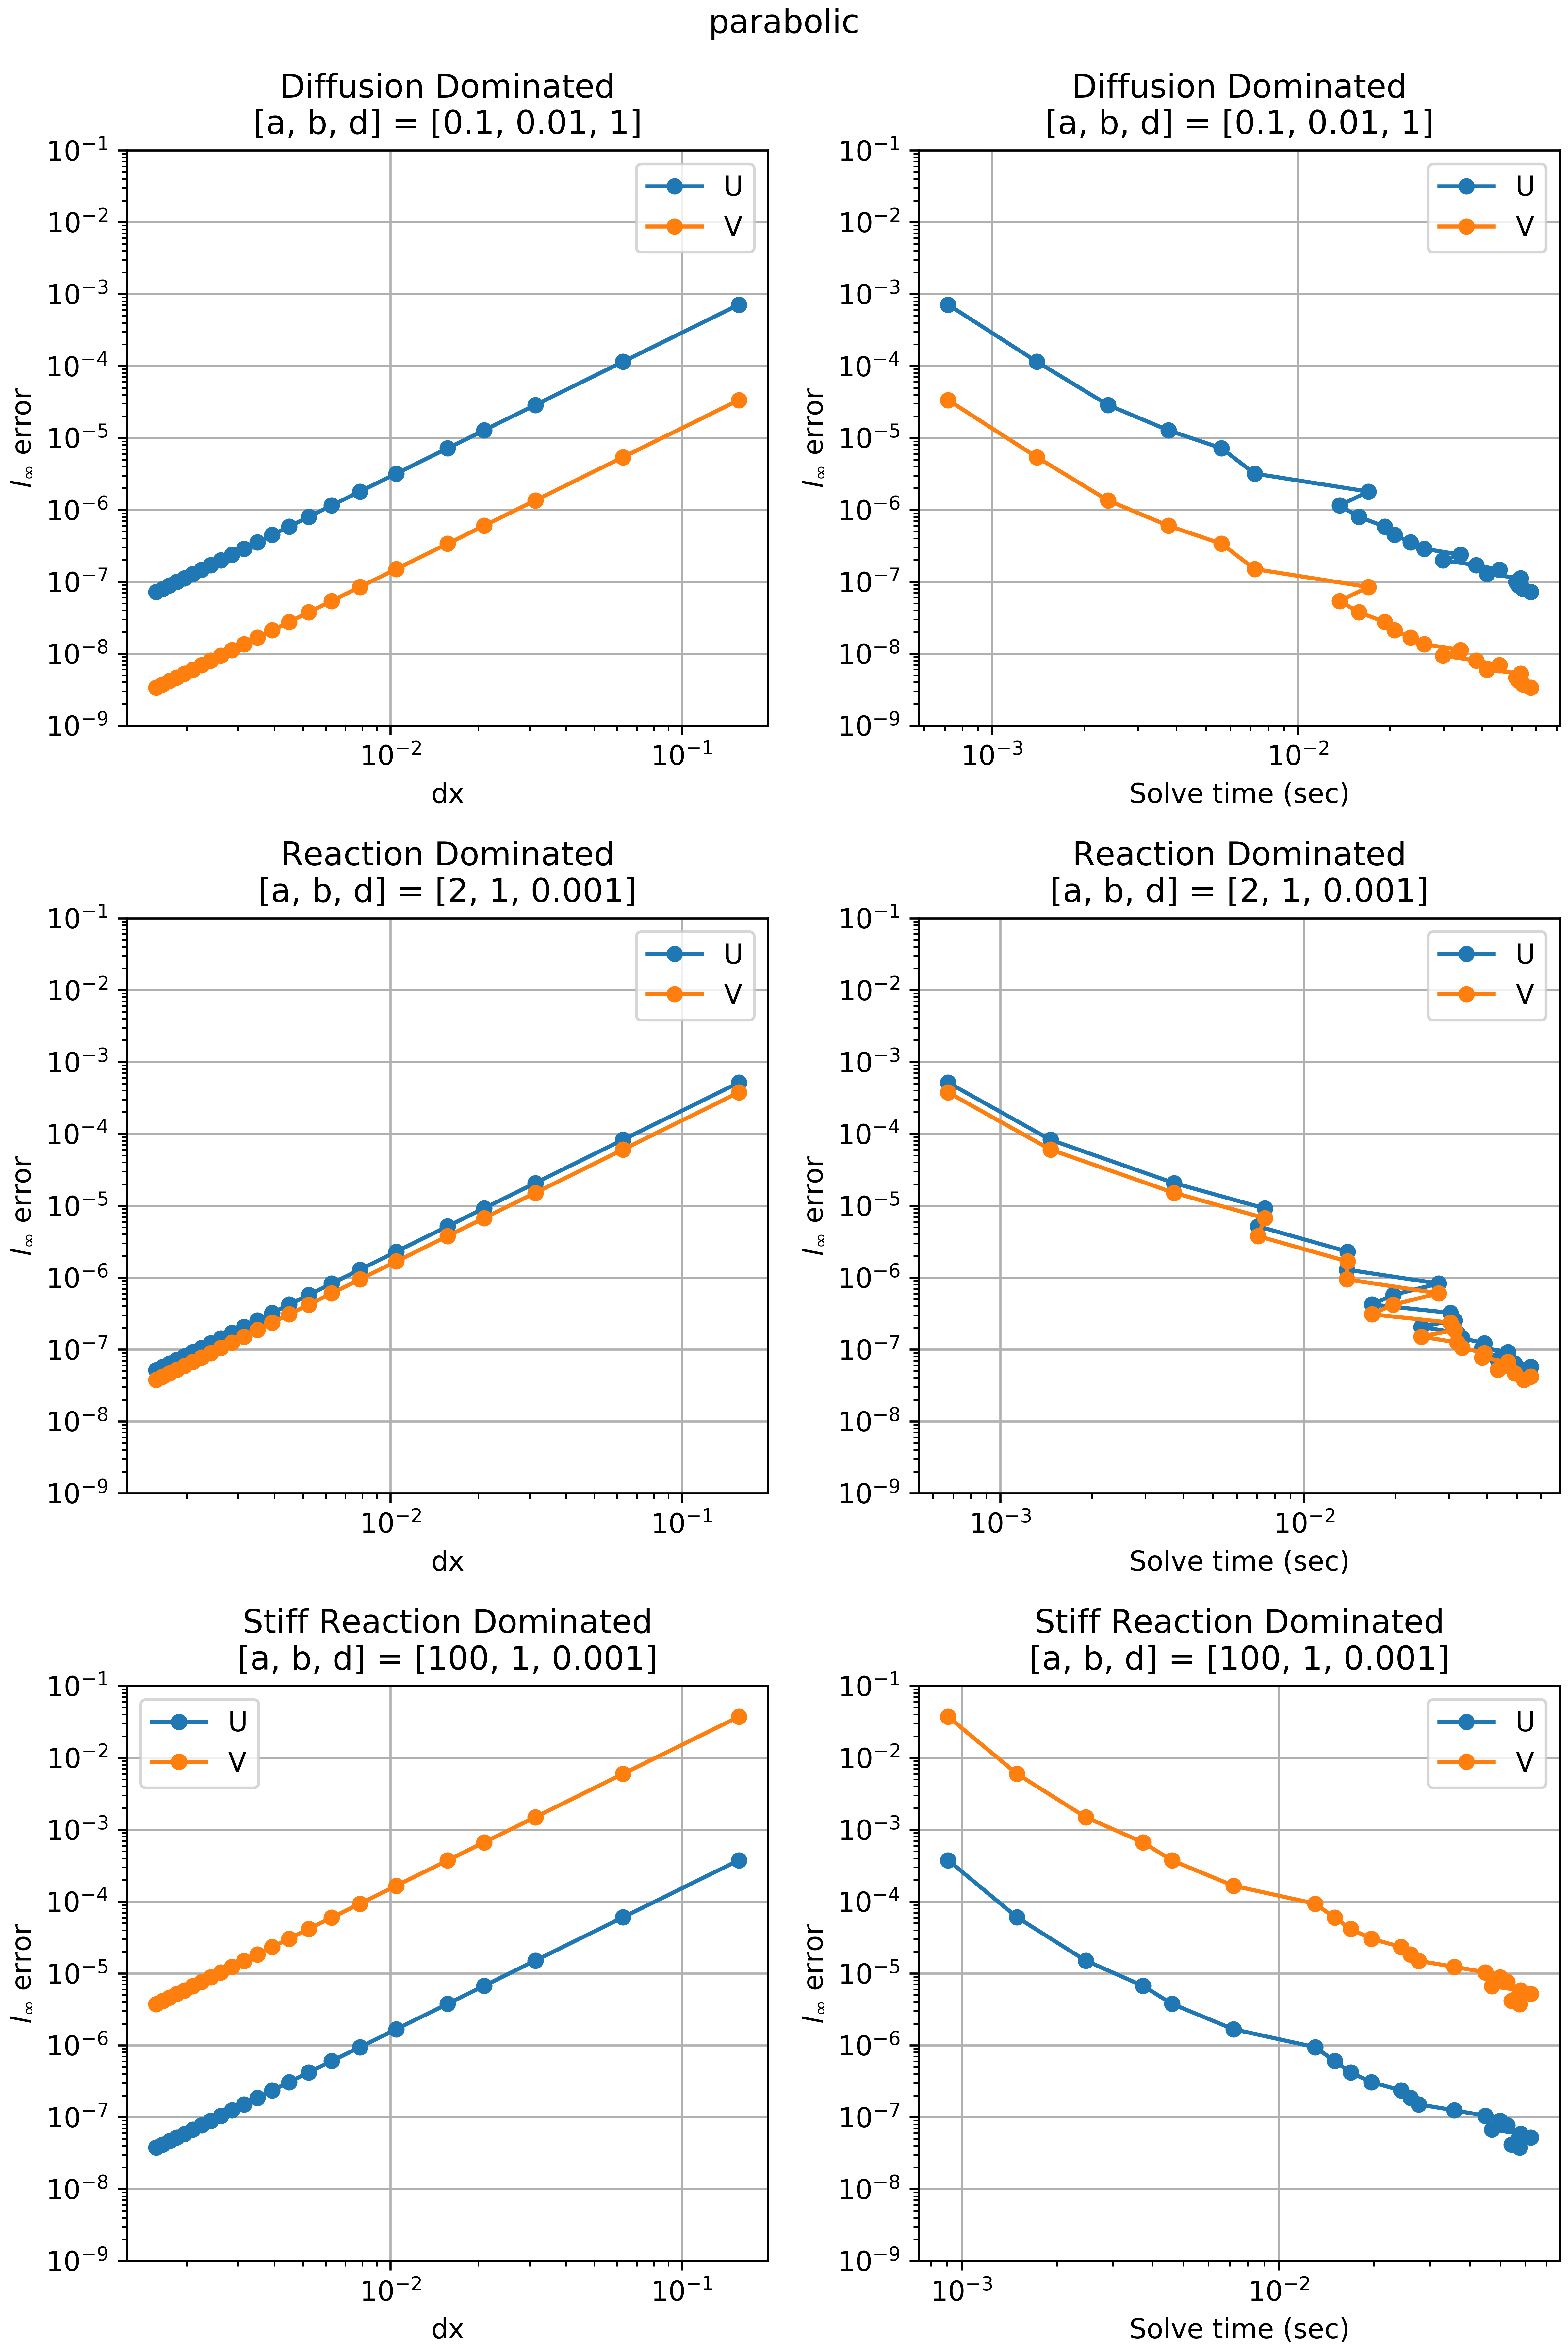
\includegraphics[width=5.75in]{images/parabolicproblem2.png}\\
  \caption{Error for Problem 2 Using Parabolic}
  \label{fig:errorProblem2parabolic}
\end{figure} 

\begin{figure}[t]
  \centering
  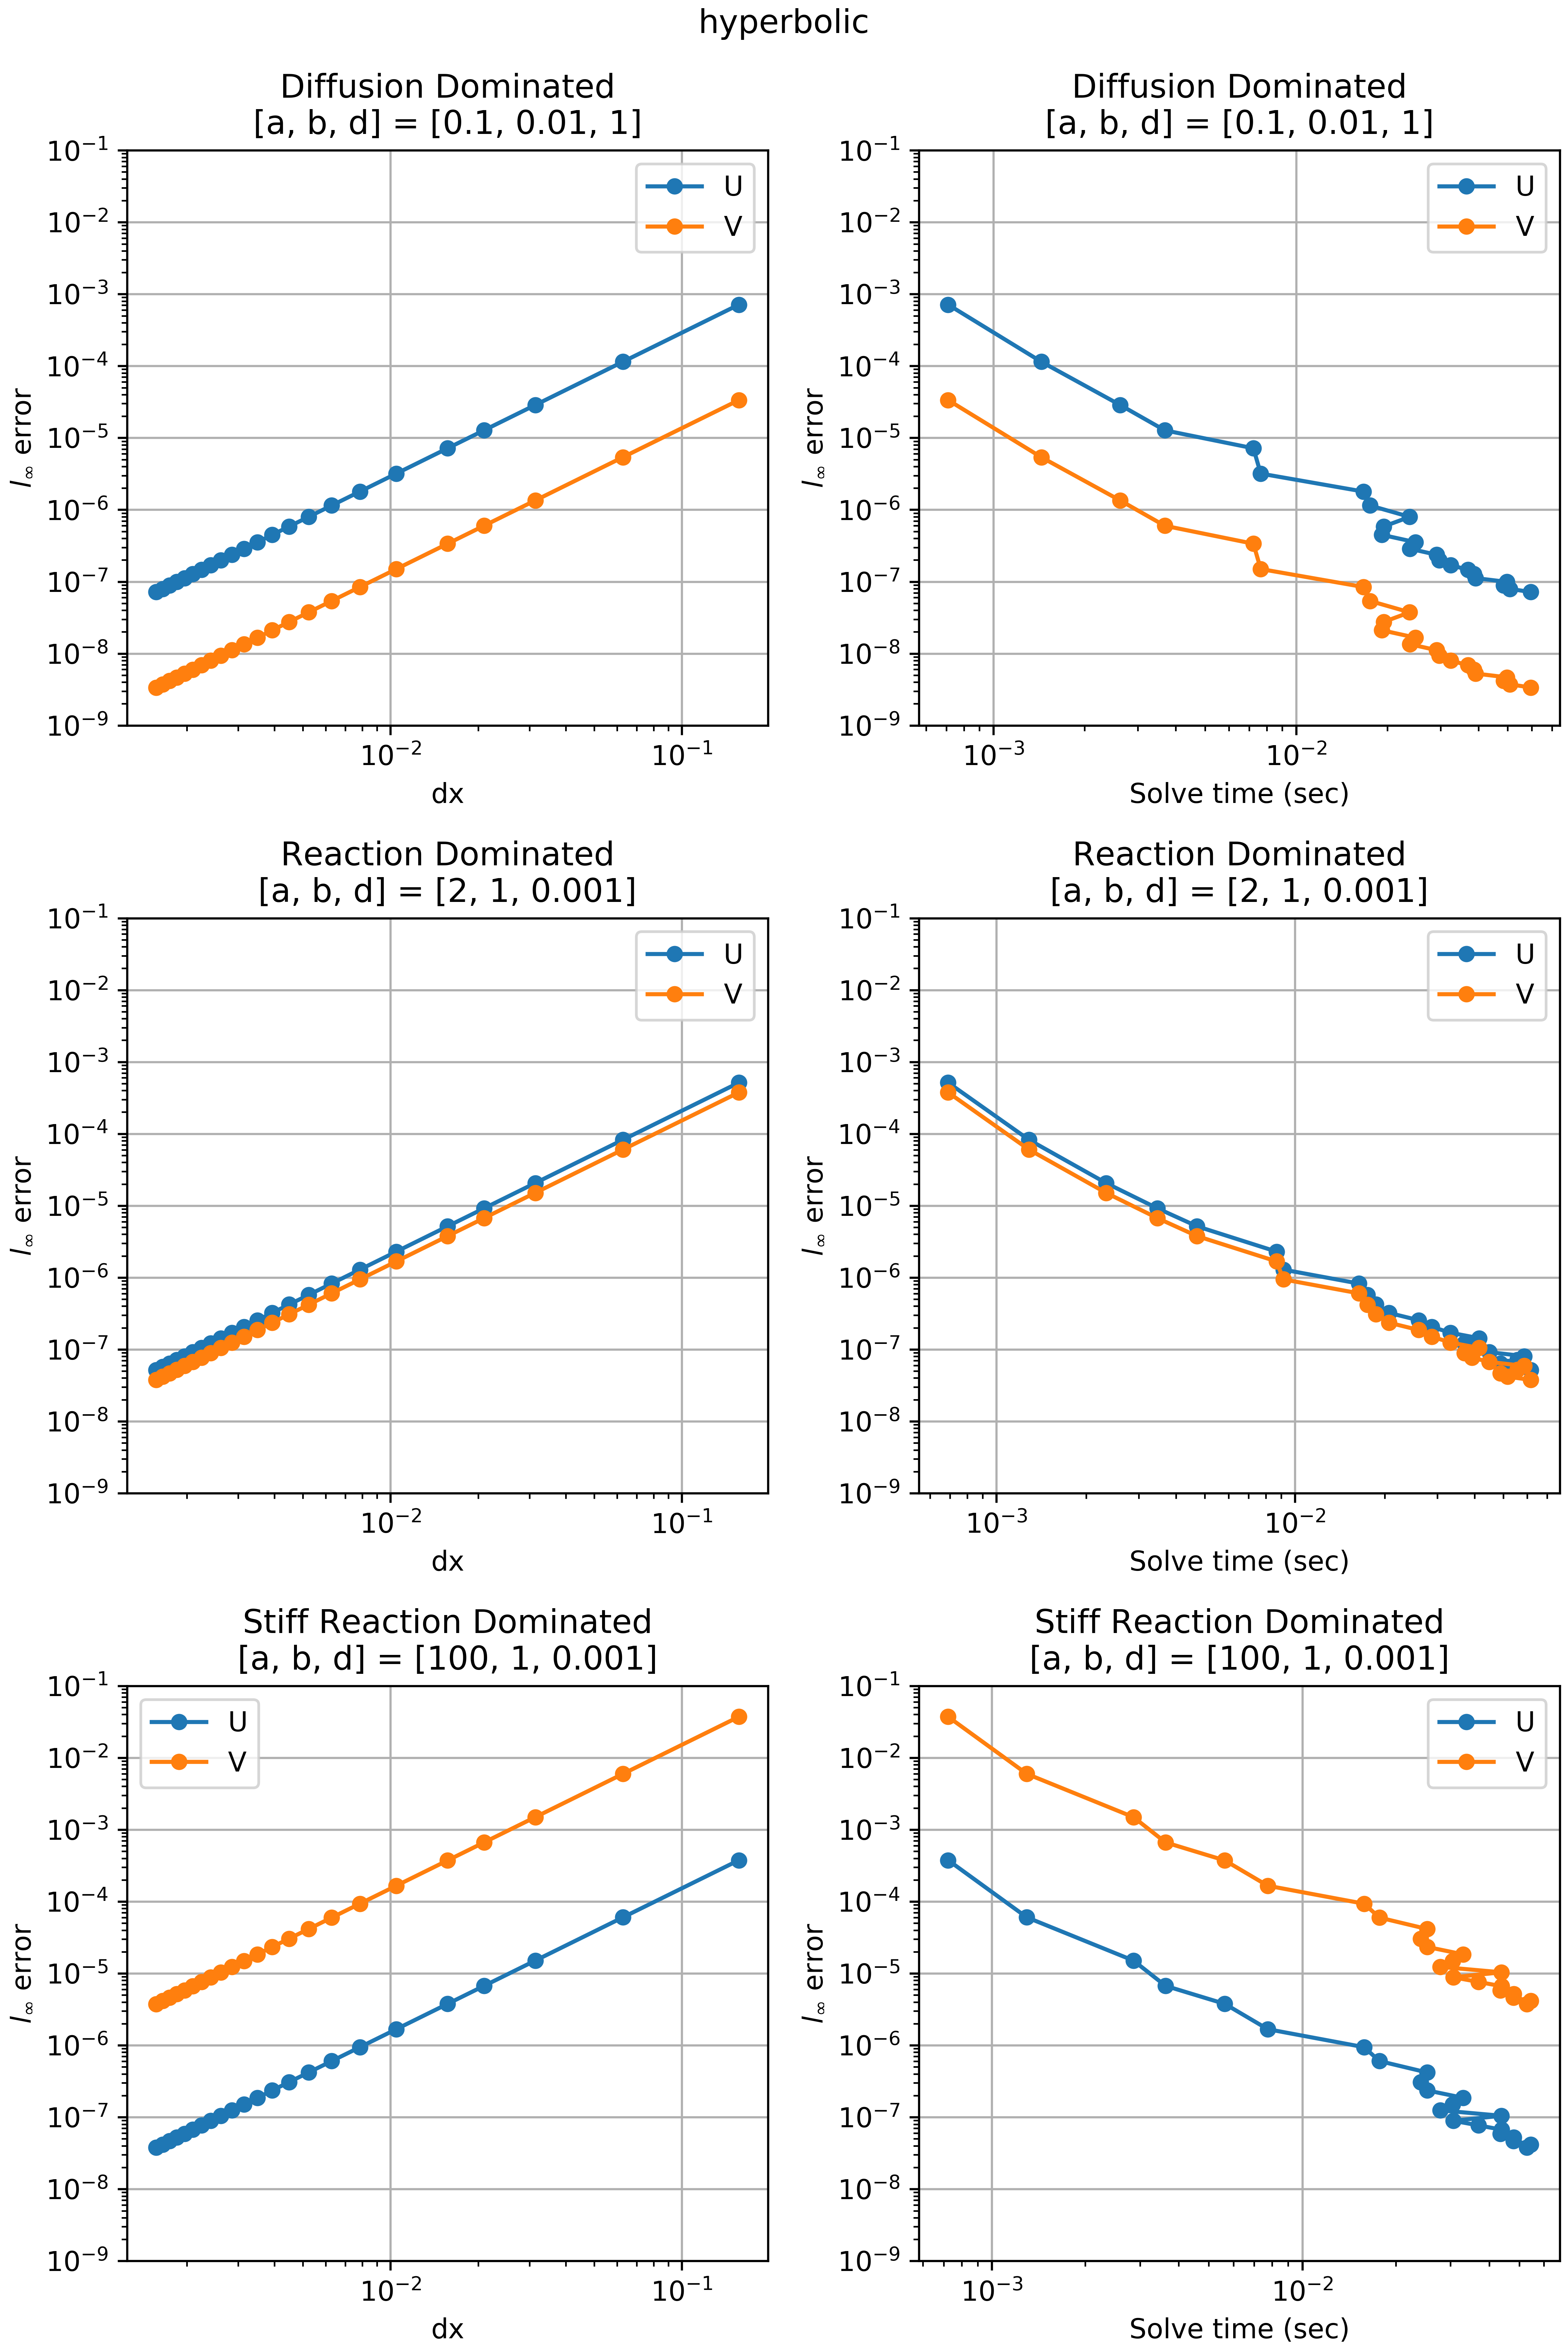
\includegraphics[width=5.75in]{images/hyperbolicproblem2.png}\\
  \caption{Error for Problem 2 Using Hyperbolic}
  \label{fig:errorProblem2hyperbolic}
\end{figure} 

\begin{figure}[t]
  \centering
  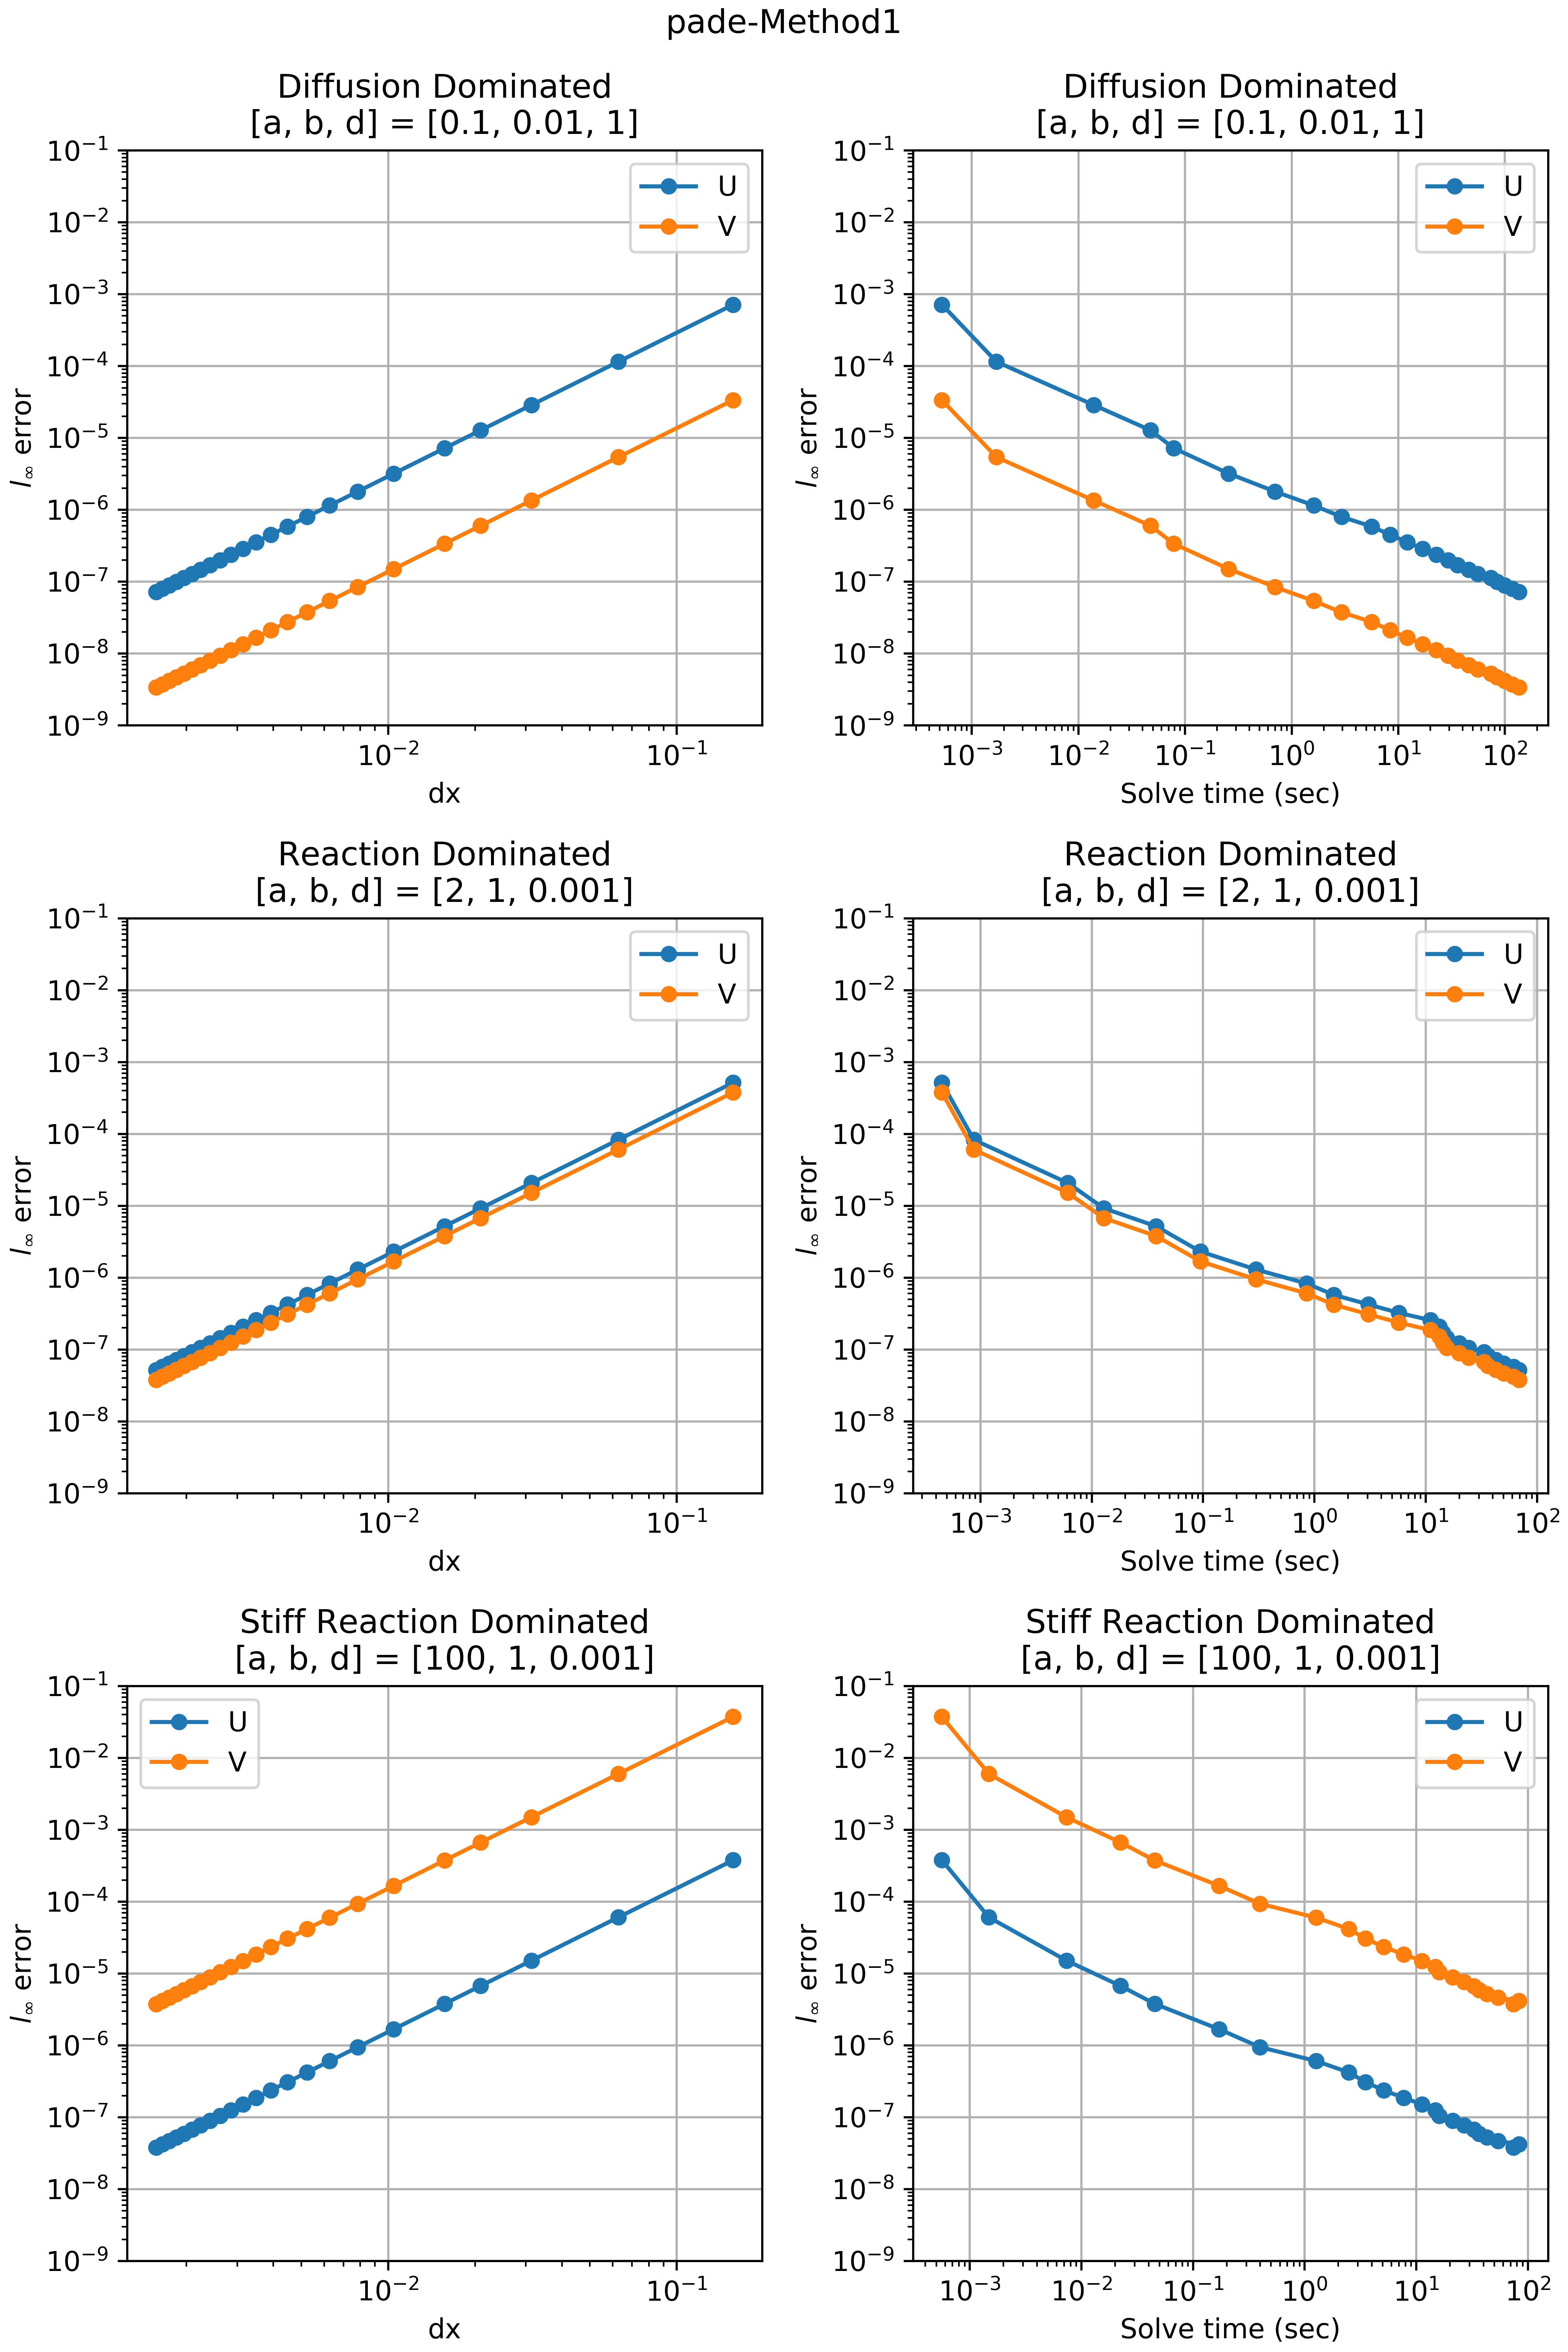
\includegraphics[width=5.75in]{images/pade-Method1problem2.png}\\
  \caption{Error for Problem 2 Using Pade-Method1}
  \label{fig:errorProblem2padeM1}
\end{figure} 

\begin{figure}[t]
  \centering
  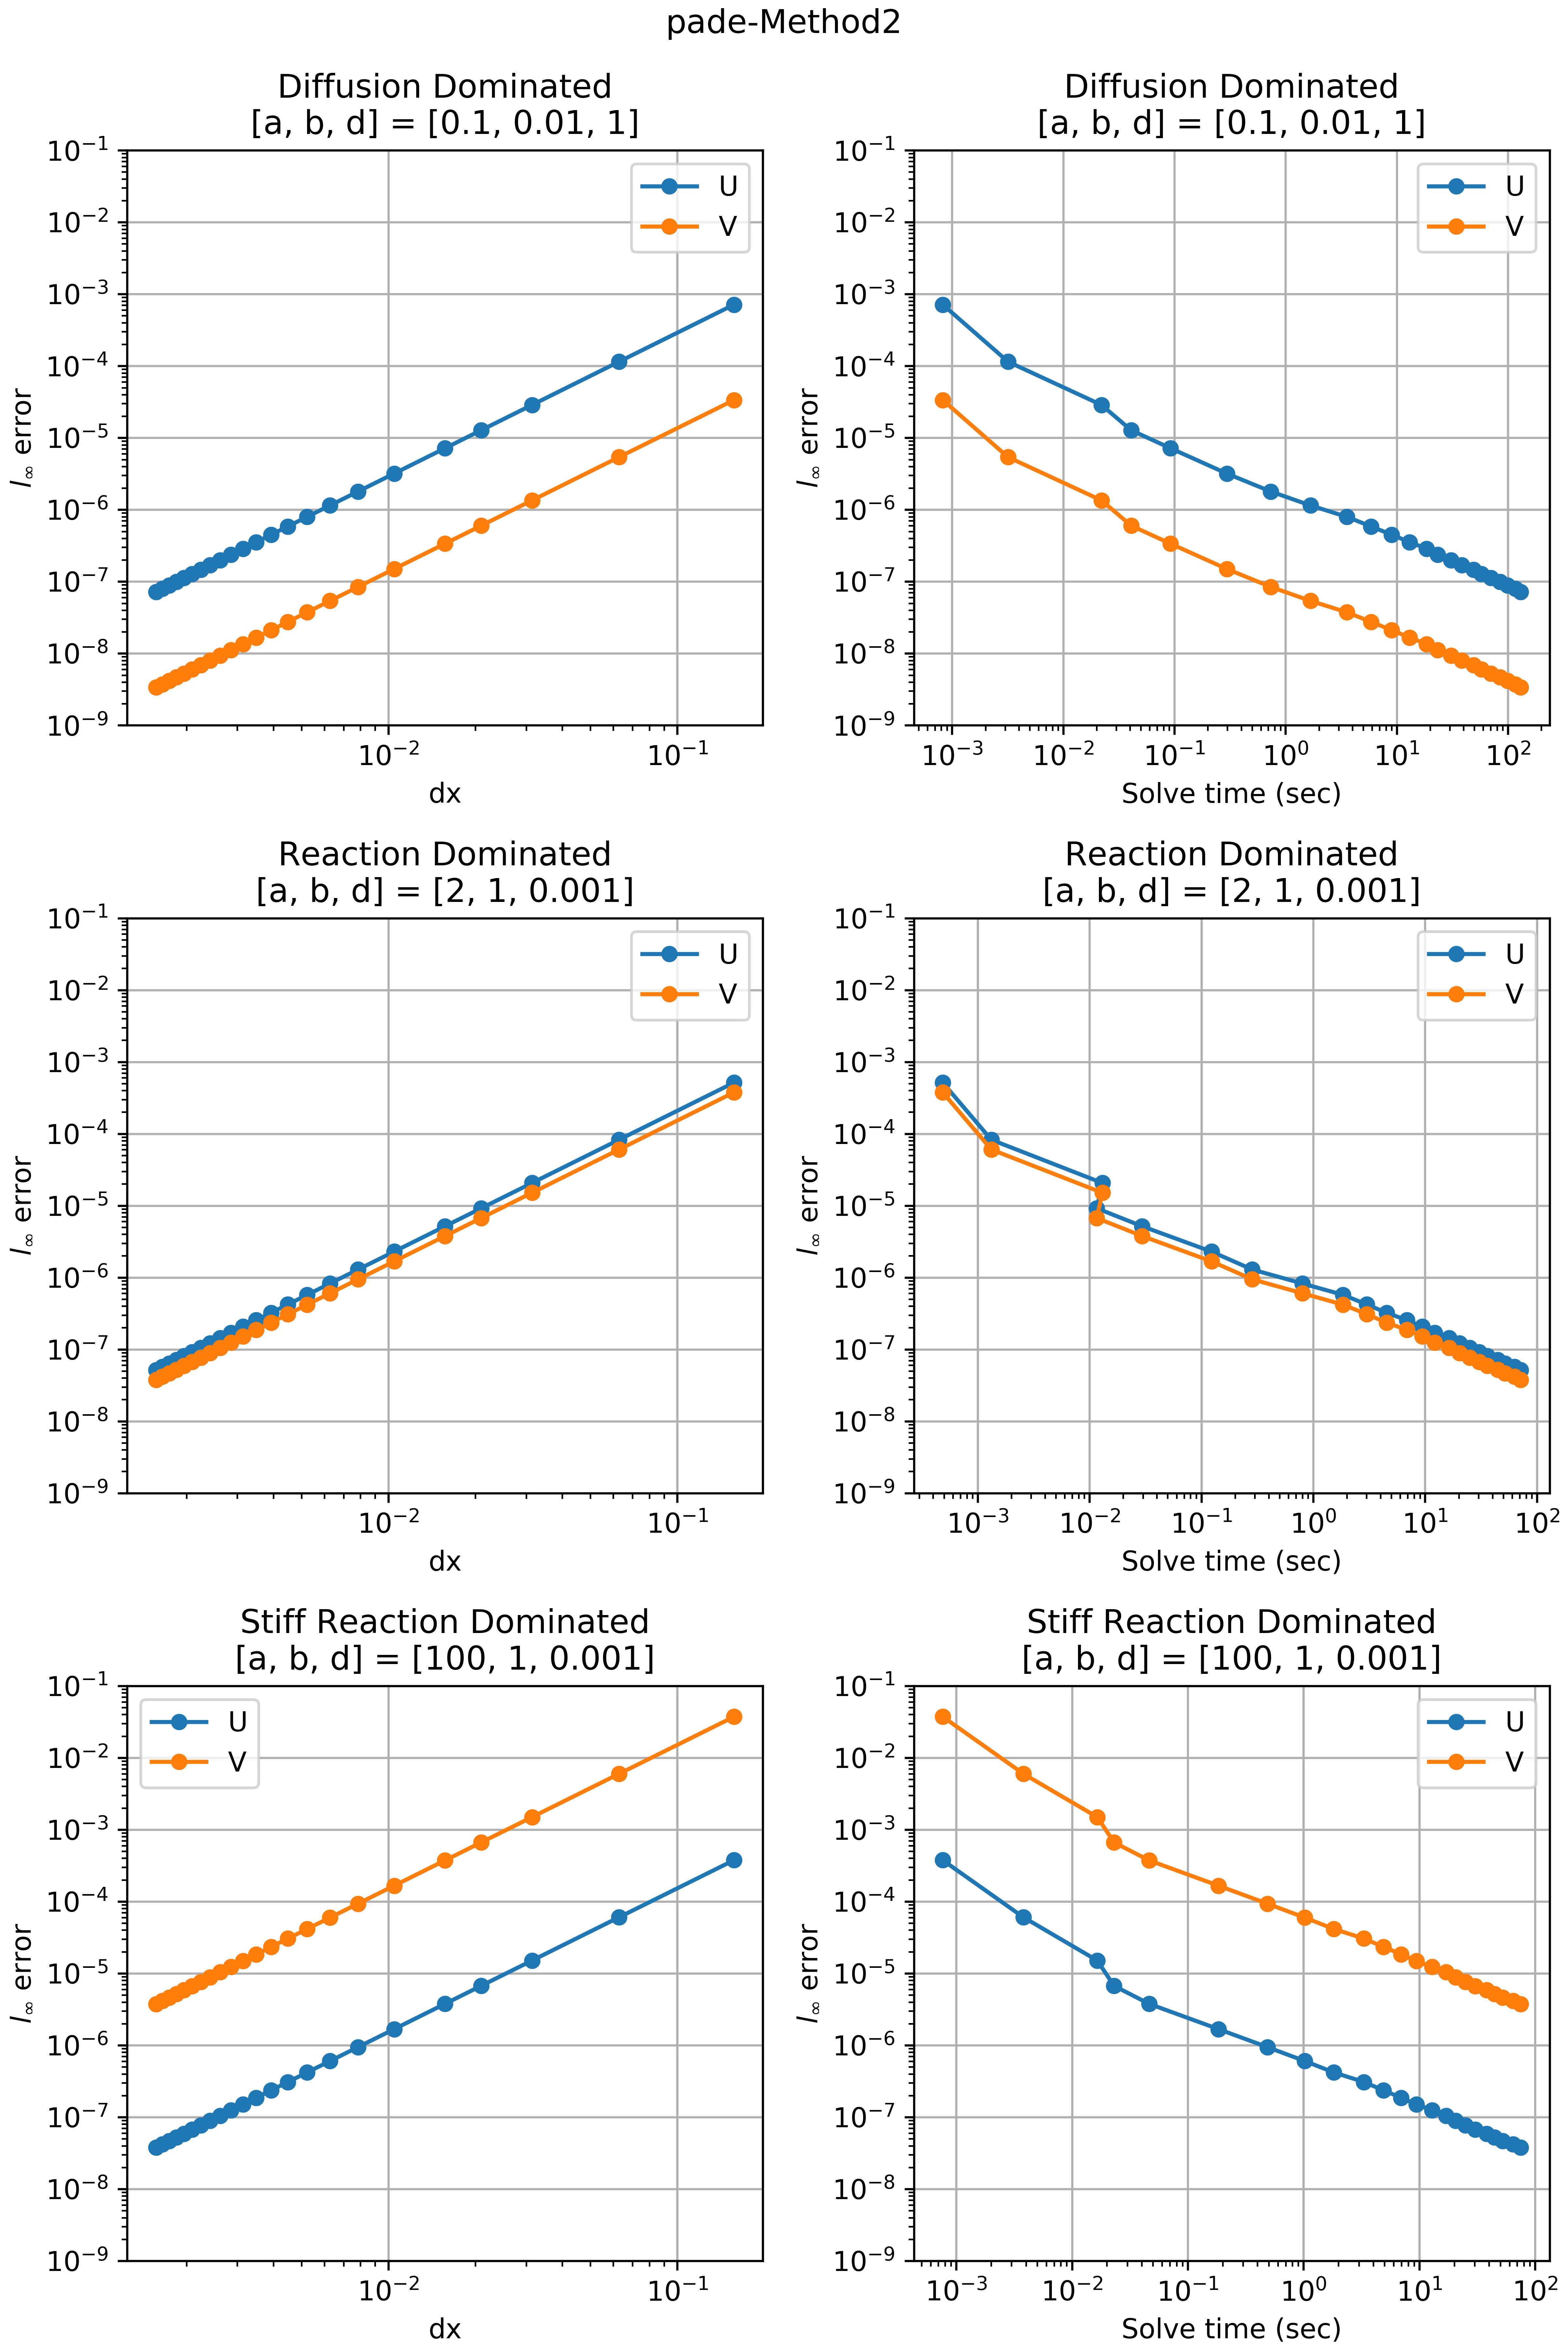
\includegraphics[width=5.75in]{images/pade-Method2problem2.png}\\
  \caption{Error for Problem 2 Using Pade-Method2}
  \label{fig:errorProblem2padeM2}
\end{figure} 

\begin{figure}[t]
  \centering
  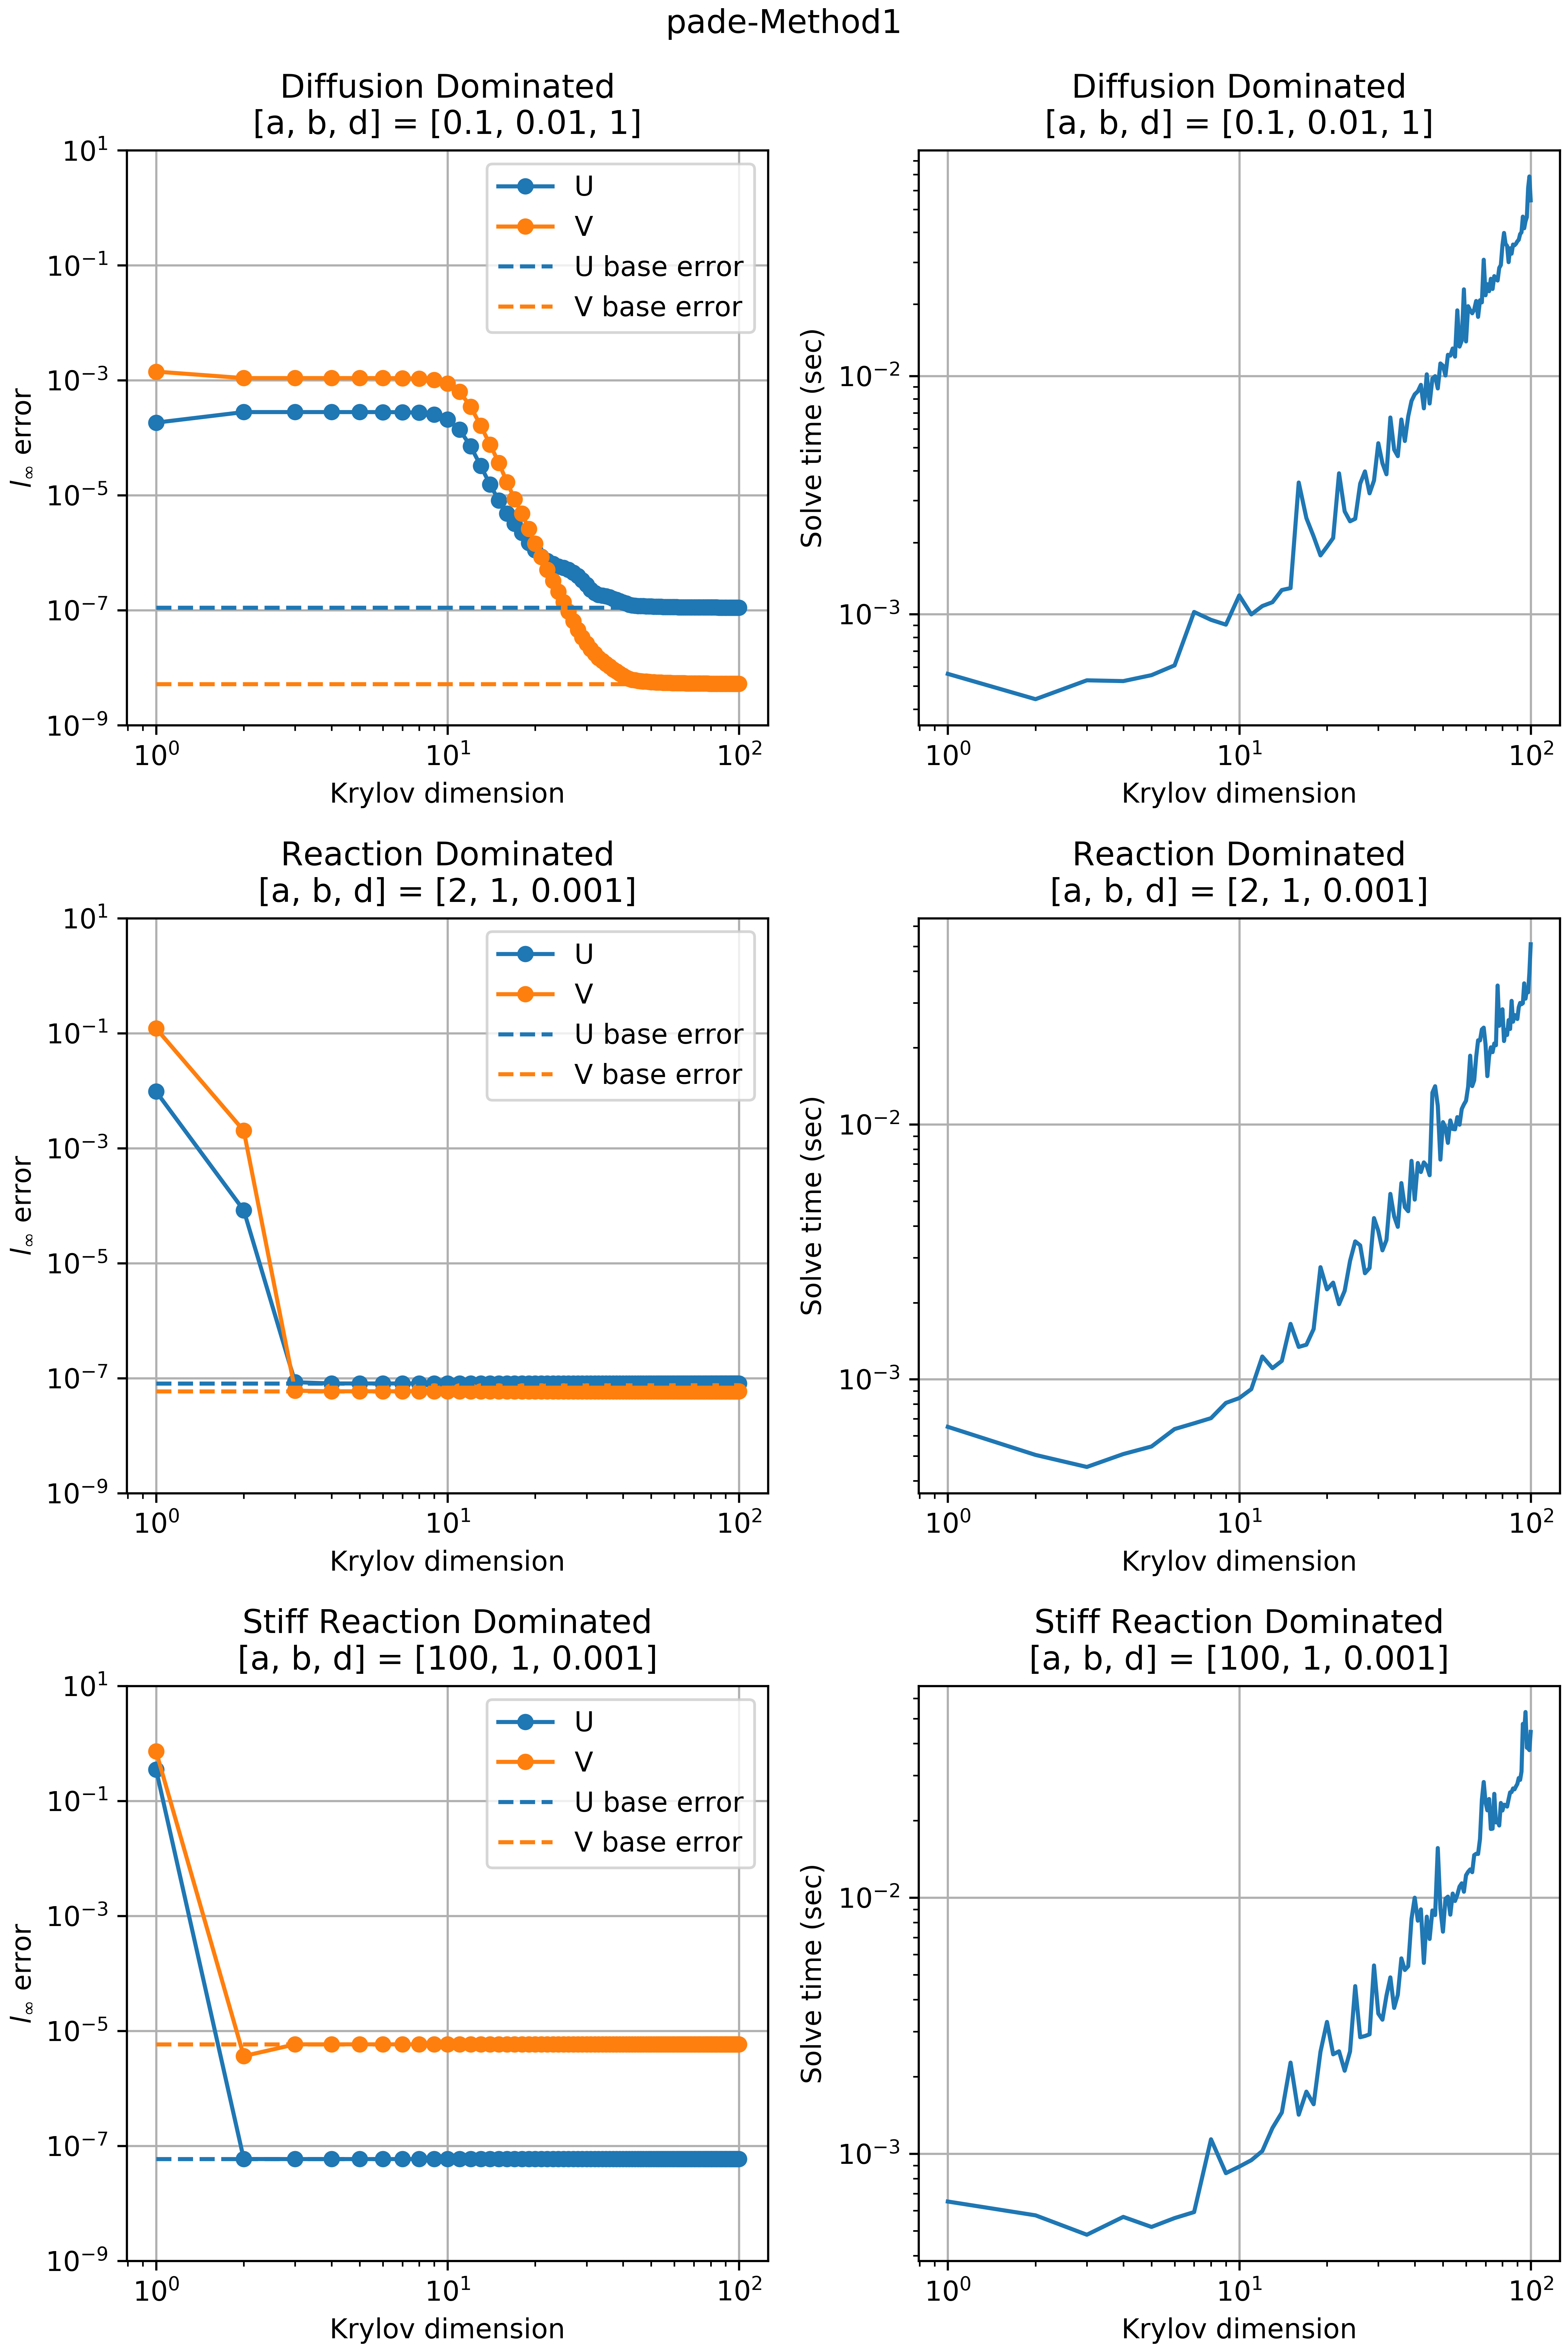
\includegraphics[width=5.75in]{images/pade-Method1KrylovProblem2.png}\\
  \caption{Krylov Approximation for Problem 2 Using Pade-Method1}
  \label{fig:errorProblem2padeM1Krylov}
\end{figure} 

\begin{figure}[t]
  \centering
  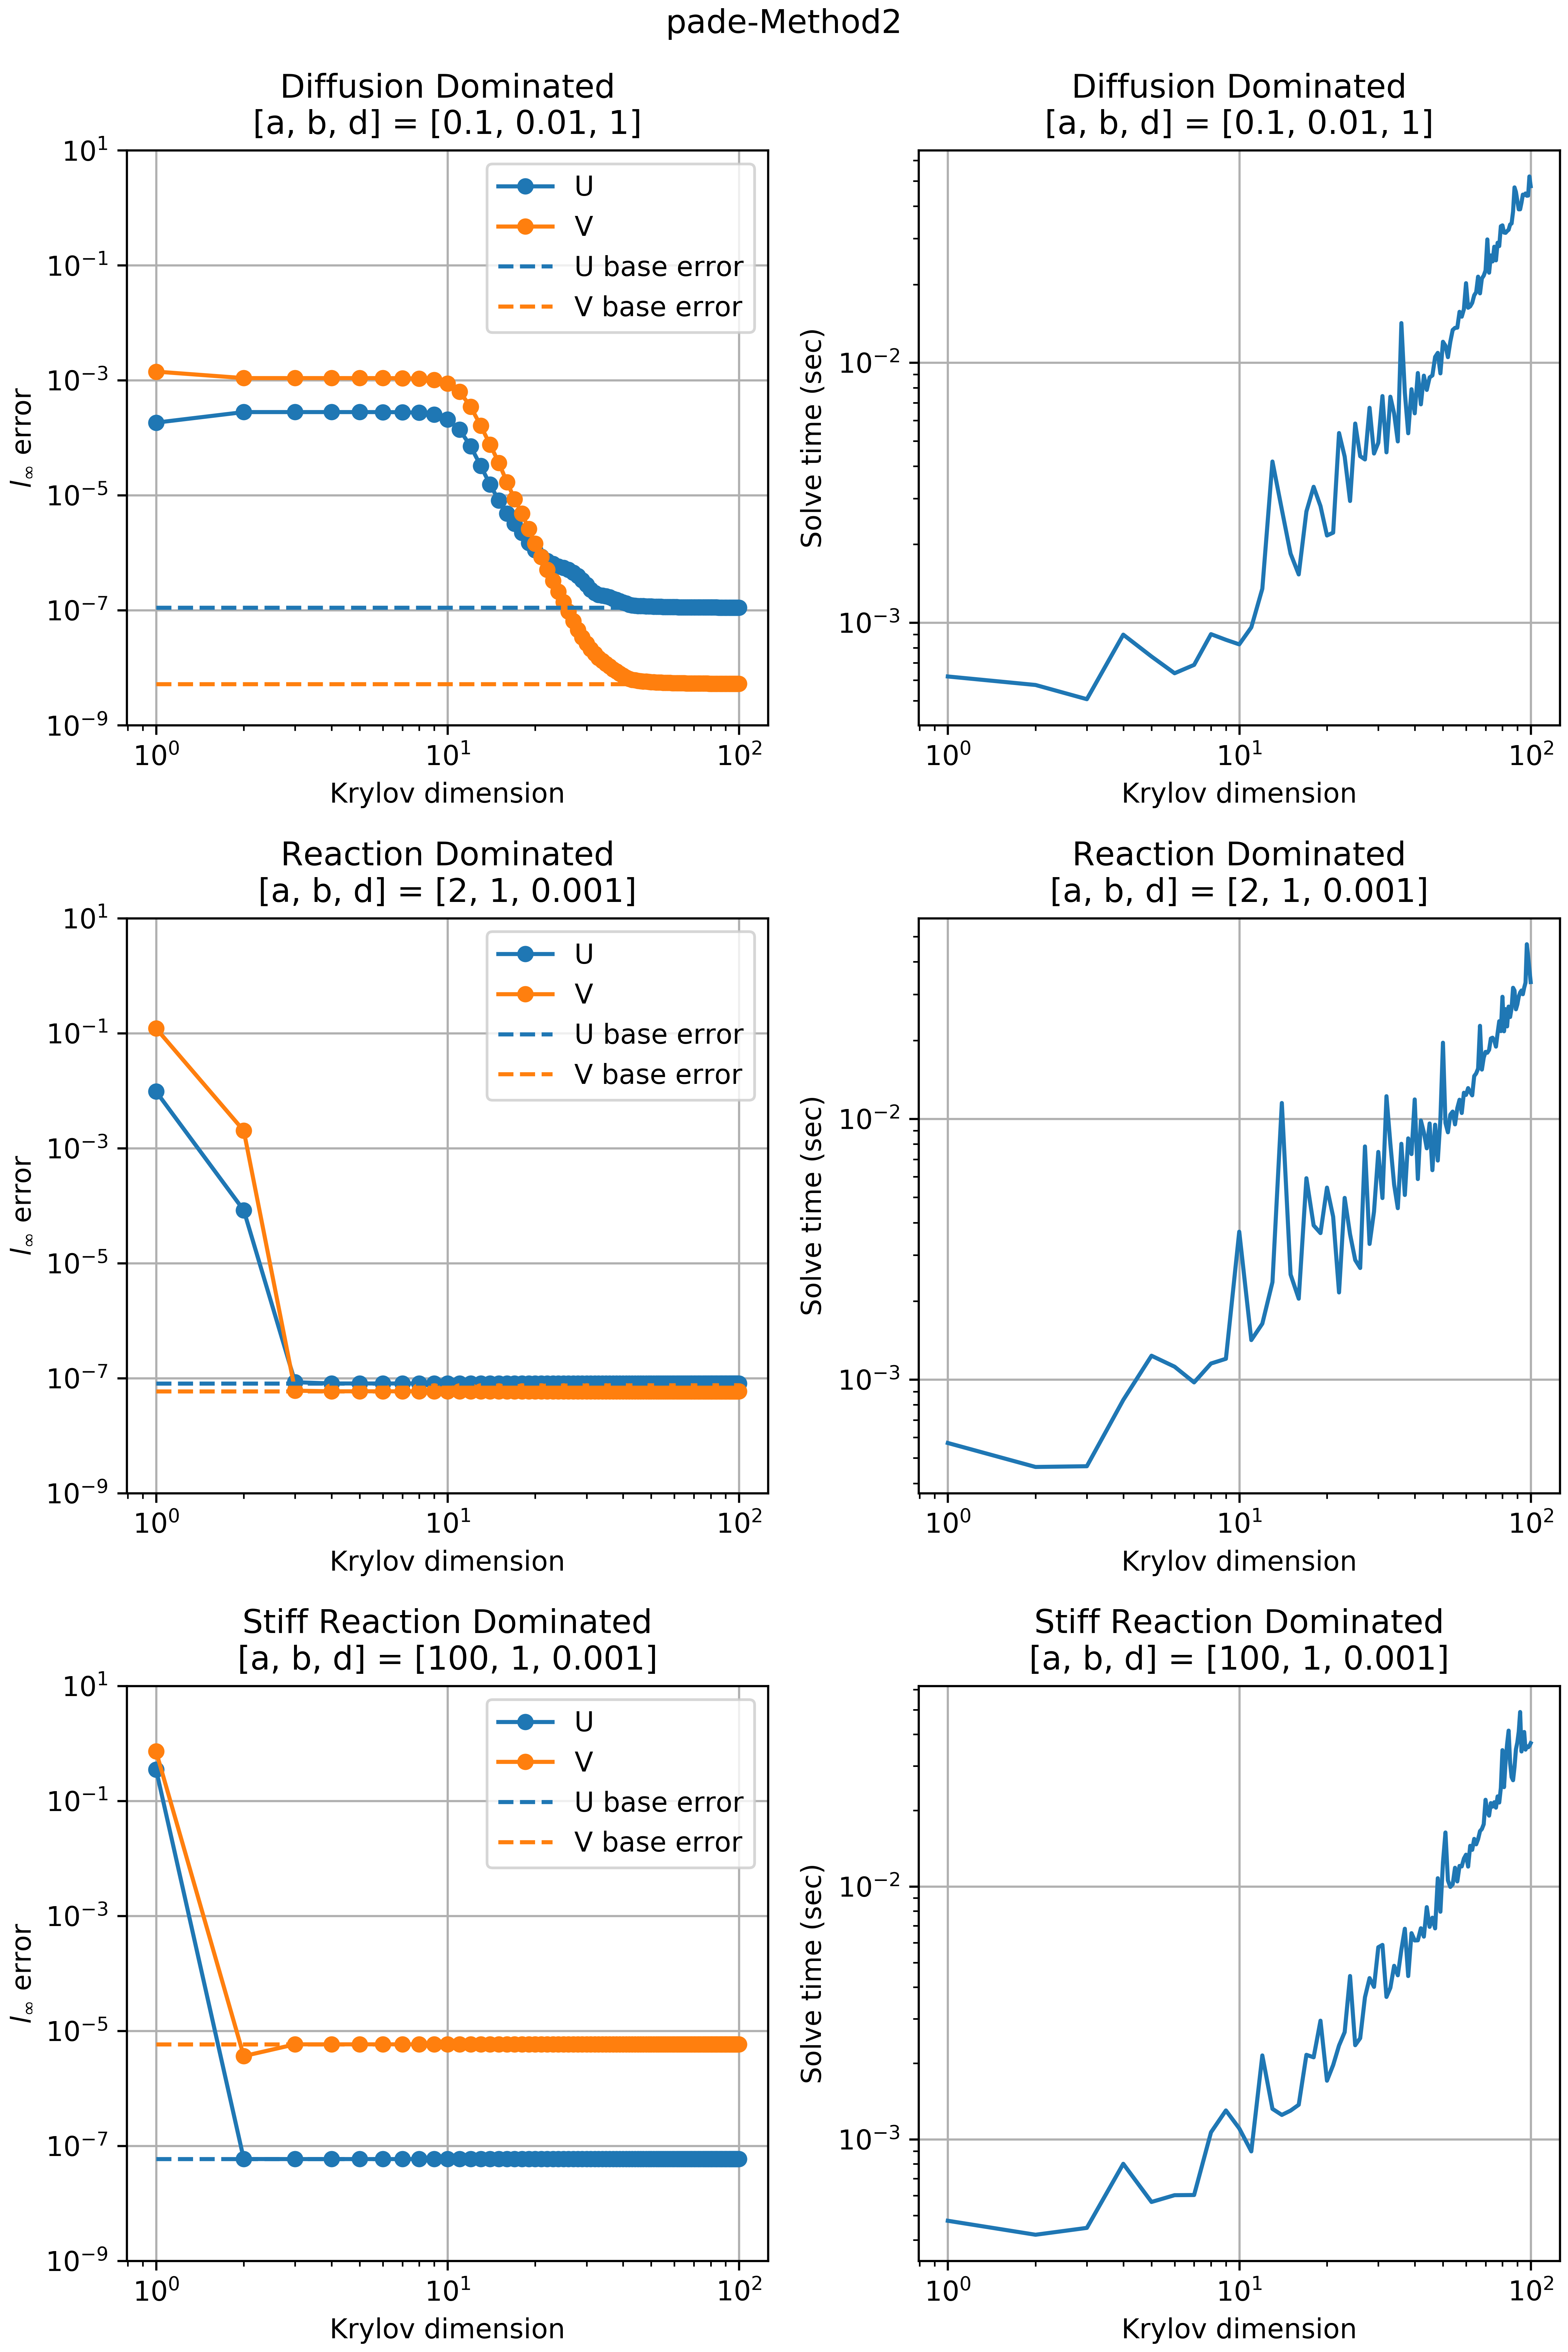
\includegraphics[width=5.75in]{images/pade-Method2KrylovProblem2.png}\\
  \caption{Krylov Approximation for Problem 2 Using Pade-Method2}
  \label{fig:errorProblem2padeM2Krylov}
\end{figure} 

\FloatBarrier


\section{Problem 3}
This problem examines a pureconvection driven flow with the 6 neutron precursor groups with xenon and iodine 135 shown in Equation \ref{eq:problem3}. 

\begin{equation}
\begin{split}
    \frac{\partial \rho_{1}}{\partial t} = -v_{y}\frac{\partial \rho_{1}}{\partial y} &- \lambda_{1}\rho_{1} + \frac{M_{1}}{N_{A}}\gamma_{1}\Sigma_{f,1}\phi, \\ 
    \frac{\partial \rho_{2}}{\partial t} = -v_{y}\frac{\partial \rho_{2}}{\partial y} &- \lambda_{2}\rho_{2} + \frac{M_{2}}{N_{A}}\gamma_{2}\Sigma_{f,2}\phi, \\ 
    \frac{\partial \rho_{3}}{\partial t} = -v_{y}\frac{\partial \rho_{3}}{\partial y} &- \lambda_{3}\rho_{3} + \frac{M_{3}}{N_{A}}\gamma_{3}\Sigma_{f,3}\phi \\
    \frac{\partial \rho_{4}}{\partial t} = -v_{y}\frac{\partial \rho_{4}}{\partial y} &- \lambda_{1}\rho_{4} + \frac{M_{4}}{N_{A}}\gamma_{1}\Sigma_{f,4}\phi \\
    \frac{\partial \rho_{5}}{\partial t} = -v_{y}\frac{\partial \rho_{5}}{\partial y} &- \lambda_{5}\rho_{5} + \frac{M_{5}}{N_{A}}\gamma_{5}\Sigma_{f,5}\phi \\
    \frac{\partial \rho_{6}}{\partial t} = -v_{y}\frac{\partial \rho_{6}}{\partial y} &- \lambda_{6}\rho_{1} + \frac{M_{6}}{N_{A}}\gamma_{6}\Sigma_{f,6}\phi \\
    \frac{\partial \rho_{Xe}}{\partial t} = -v_{y}\frac{\partial \rho_{Xe}}{\partial y} - \lambda_{Xe}&\rho_{Xe} + \frac{M_{Xe}}{M_{I}}\lambda_{I}\rho_{I} +  \frac{M_{I}}{N_{A}}\gamma_{I}\Sigma_{f,Xe}\phi \\
    \frac{\partial \rho_{I}}{\partial t} = -v_{y}\frac{\partial \rho_{I}}{\partial y} &- \lambda_{I}\rho_{I} + \frac{M_{I}}{N_{A}}\gamma_{I}\Sigma_{f,I}\phi
\end{split}
\label{eq:problem3}
\end{equation}